\subsection{Recognising obstacle height (Q2)}
\label{sec:res-height}

\subsubsection{Generic models versus person scaling}

Table~\ref{tab:limbs} is the central result. A \emph{generic} model (features referenced only to the person's level walk)
recognises the height of an unseen person's obstacle in 56--62\,\% of cases (chance 33\,\%). Scaling the features with the
person's own crossings (no labels) raises this to 80--90\,\%, the best being separate random forests for the leading and
trailing limb combined by soft vote: 90.0\,\% (85--95). The same holds for the six obstacles (29--30\,\% generic, 61\,\% with
person scaling; chance 17\,\%). Width stays close to chance with every setting (Section~\ref{sec:res-width}).

\begin{table}[htbp]
\centering
\caption{Height, width and the six obstacles from all Dot features of the leading limb, the trailing limb, or both (soft vote);
level-walk (generic) vs person (self) scaling; logistic regression vs random forest. Balanced accuracy (95\,\% CI).}
\label{tab:limbs}
\begin{adjustbox}{max width=\textwidth}
{\footnotesize
\begin{tabular}{lrllrrr}
\toprule
\textbf{target} & \textbf{chance} & \textbf{norm} & \textbf{model} & \textbf{lead} & \textbf{trail} & \textbf{fusion (lead + trail vote)} \\
\midrule
height & 33\% & level & logreg & 62.1\% (55--70) & 49.1\% (40--58) & 56.1\% (46--66) \\
height & 33\% & level & forest & 59.3\% (50--68) & 59.2\% (48--71) & 60.4\% (49--73) \\
height & 33\% & self & logreg & 79.6\% (73--86) & 78.0\% (67--87) & 80.8\% (74--87) \\
height & 33\% & self & forest & 87.6\% (82--92) & 86.1\% (79--92) & 90.0\% (85--95) \\
width & 50\% & level & logreg & 54.1\% (49--59) & 57.0\% (51--63) & 56.1\% (52--60) \\
width & 50\% & level & forest & 61.0\% (55--69) & 54.8\% (51--59) & 58.7\% (53--66) \\
width & 50\% & self & logreg & 64.6\% (63--67) & 58.5\% (53--65) & 64.3\% (59--69) \\
width & 50\% & self & forest & 61.9\% (58--66) & 56.9\% (53--61) & 59.2\% (54--64) \\
6 obstacles & 17\% & level & logreg & 28.6\% (22--35) & 27.5\% (24--32) & 29.1\% (23--35) \\
6 obstacles & 17\% & level & forest & 30.8\% (24--38) & 29.7\% (24--36) & 30.2\% (24--37) \\
6 obstacles & 17\% & self & logreg & 45.4\% (40--51) & 38.0\% (29--47) & 45.3\% (40--51) \\
6 obstacles & 17\% & self & forest & 49.8\% (42--58) & 57.9\% (51--66) & 61.2\% (54--69) \\
\bottomrule
\end{tabular}
}
\end{adjustbox}

\end{table}

Figure~\ref{fig:limbs} shows the same comparison for logistic regression, with two tasks the Dot solves almost perfectly: which
limb a swing belongs to, and whether a stride crosses an obstacle (Tables~\ref{tab:leadtrail} and \ref{tab:obslevel}). The generic
model's errors are almost all between neighbouring heights (Figure~\ref{fig:confusion}): H1 and H3 are confused in only 4 of 170
crossings, but the middle height H2 is recognised in only 39\,\% of cases (50\,\% with the leading limb alone). More training
participants would not close the gap (Figure~\ref{fig:learning}): with all features the generic model stays at 54--57\,\% from 2 to
9 training participants, and the leading-limb models gain at most 2 points from 6 to 9 participants. The limit of the generic
model is the difference between people, not the amount of data.

\begin{figure}[htbp]
\centering
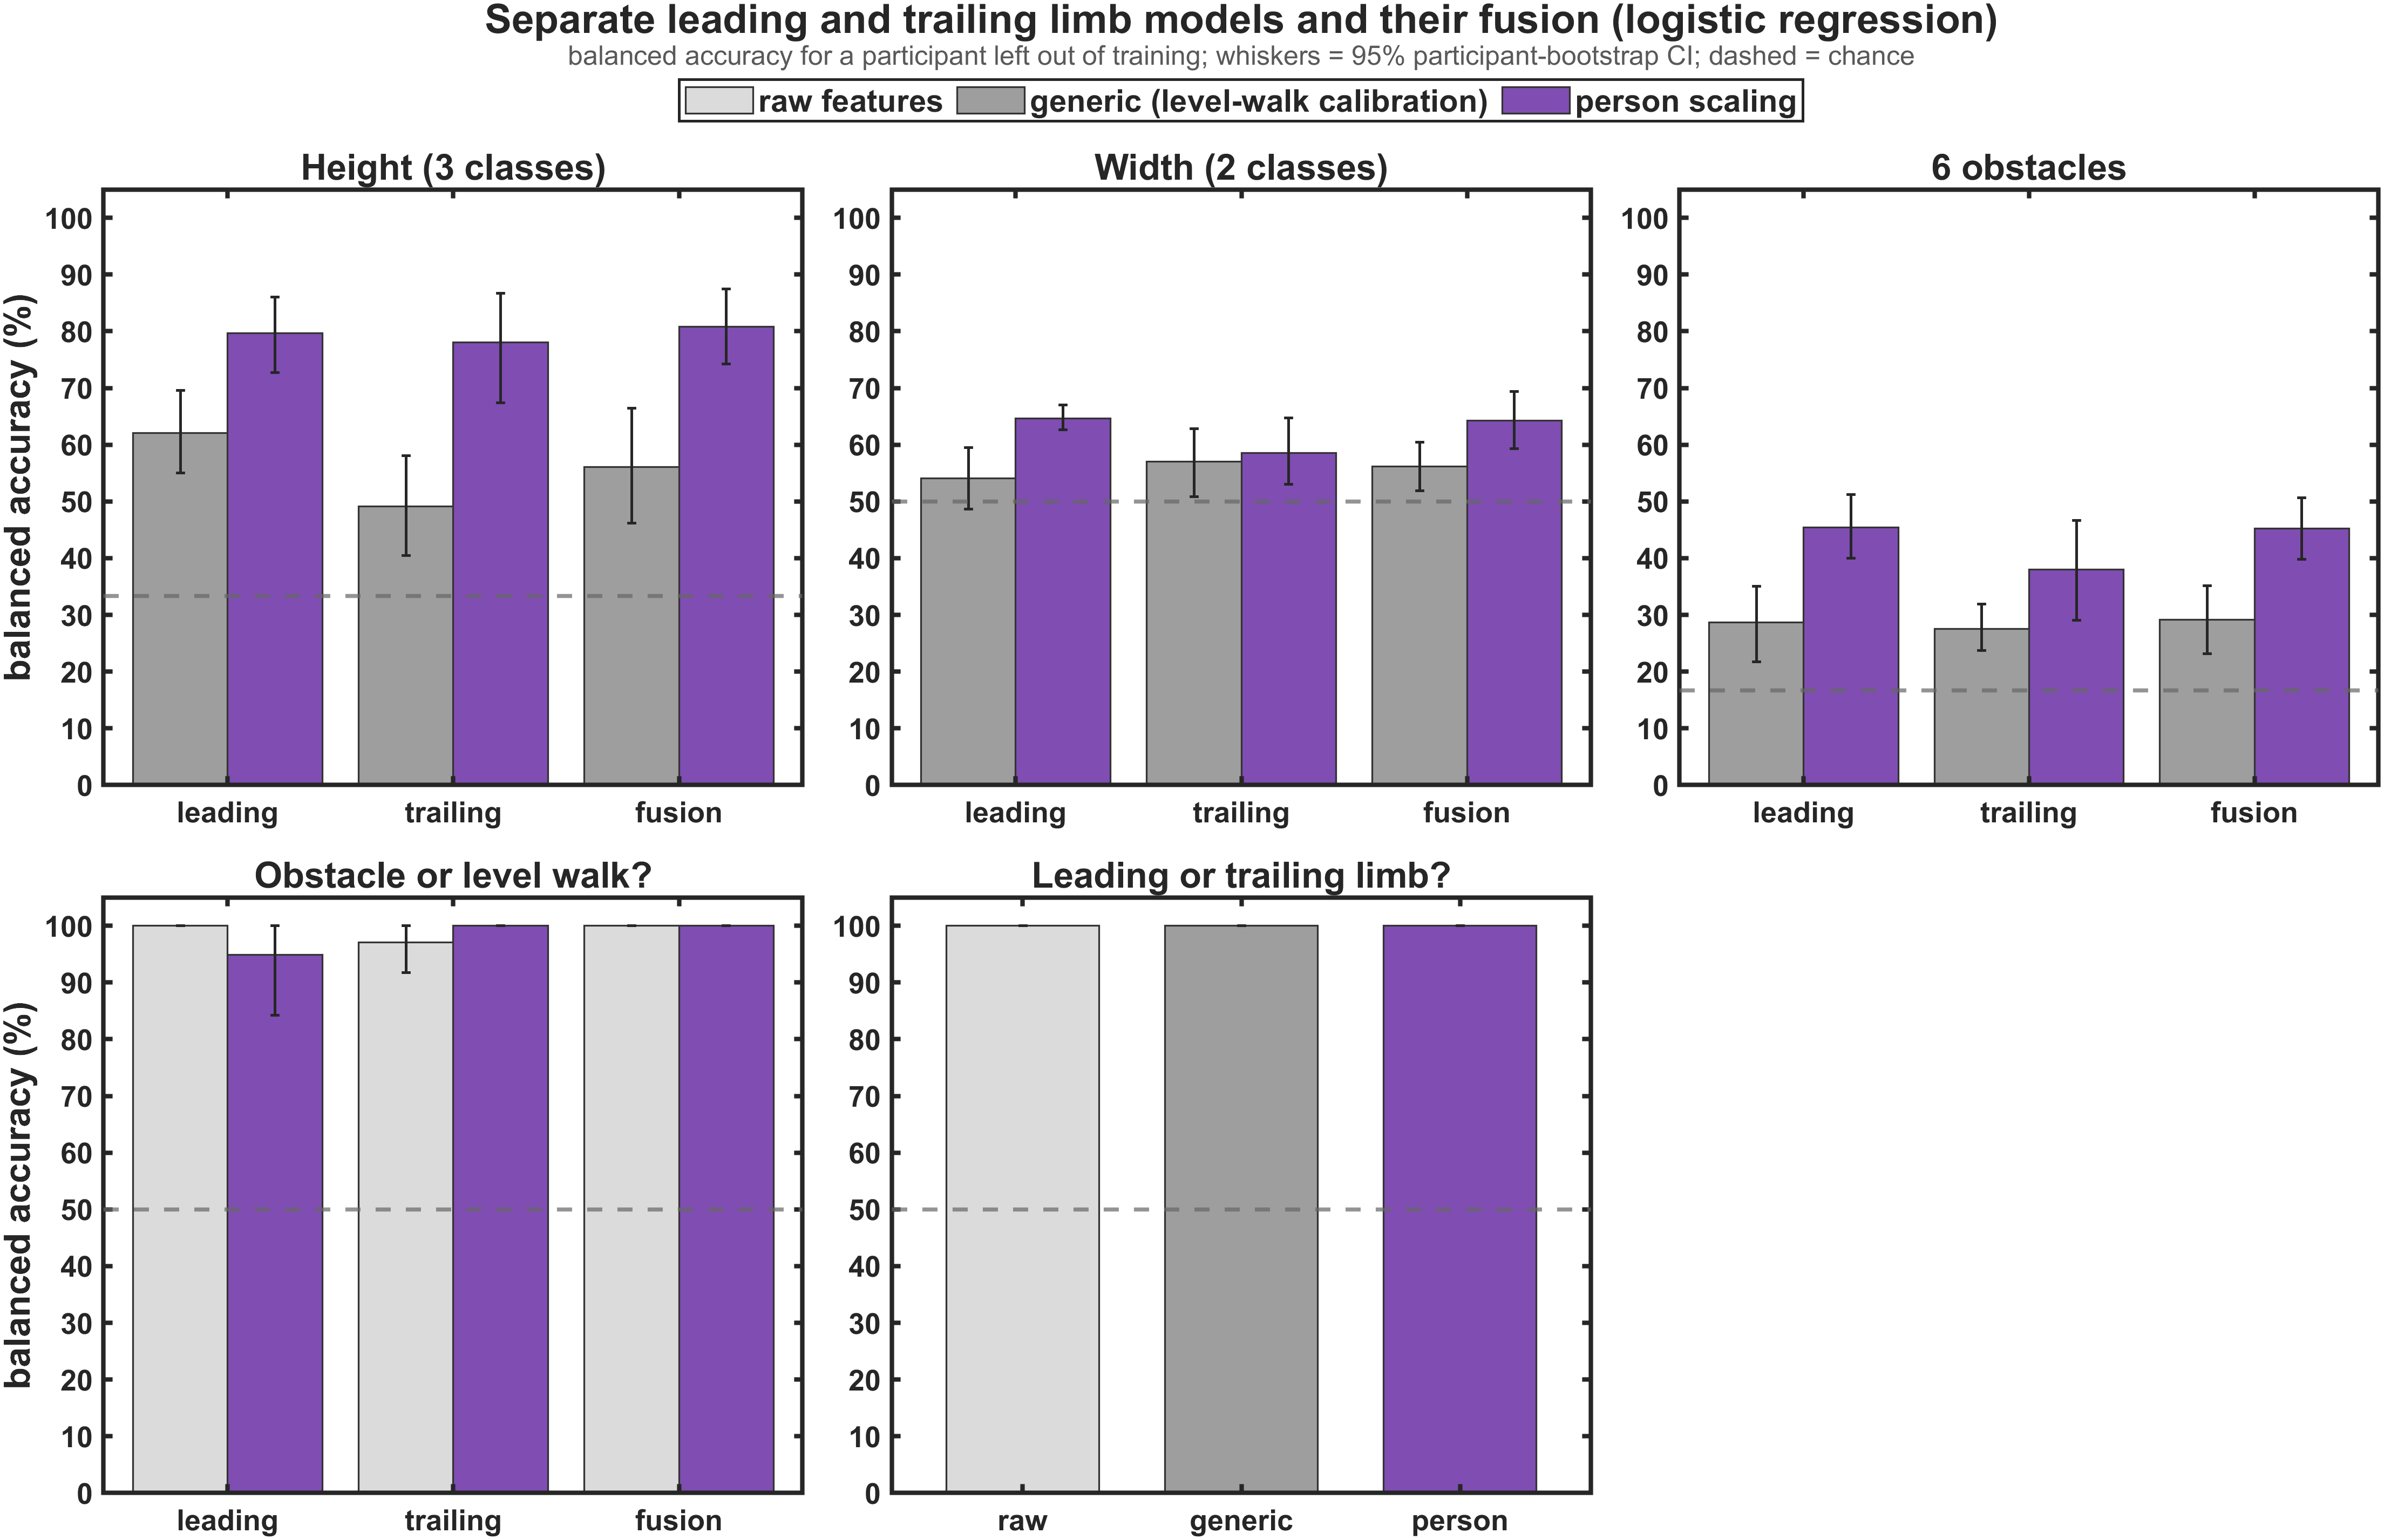
\includegraphics[width=\textwidth]{fig_limbs.png}
\caption{Separate models for the leading and the trailing limb and their soft-vote fusion (logistic regression): obstacle height, width
and the six obstacles, obstacle crossing versus level-walk stride, and which limb a swing belongs to. Bar colour = scaling: raw
features (light grey), generic level-walk calibration (grey), person scaling (purple). Whiskers = 95\,\% participant-bootstrap
CI; dashed = chance. Source: \vn{crossing_ml_matlab.m}, part 3.}
\label{fig:limbs}
\end{figure}

\begin{figure}[htbp]
\centering
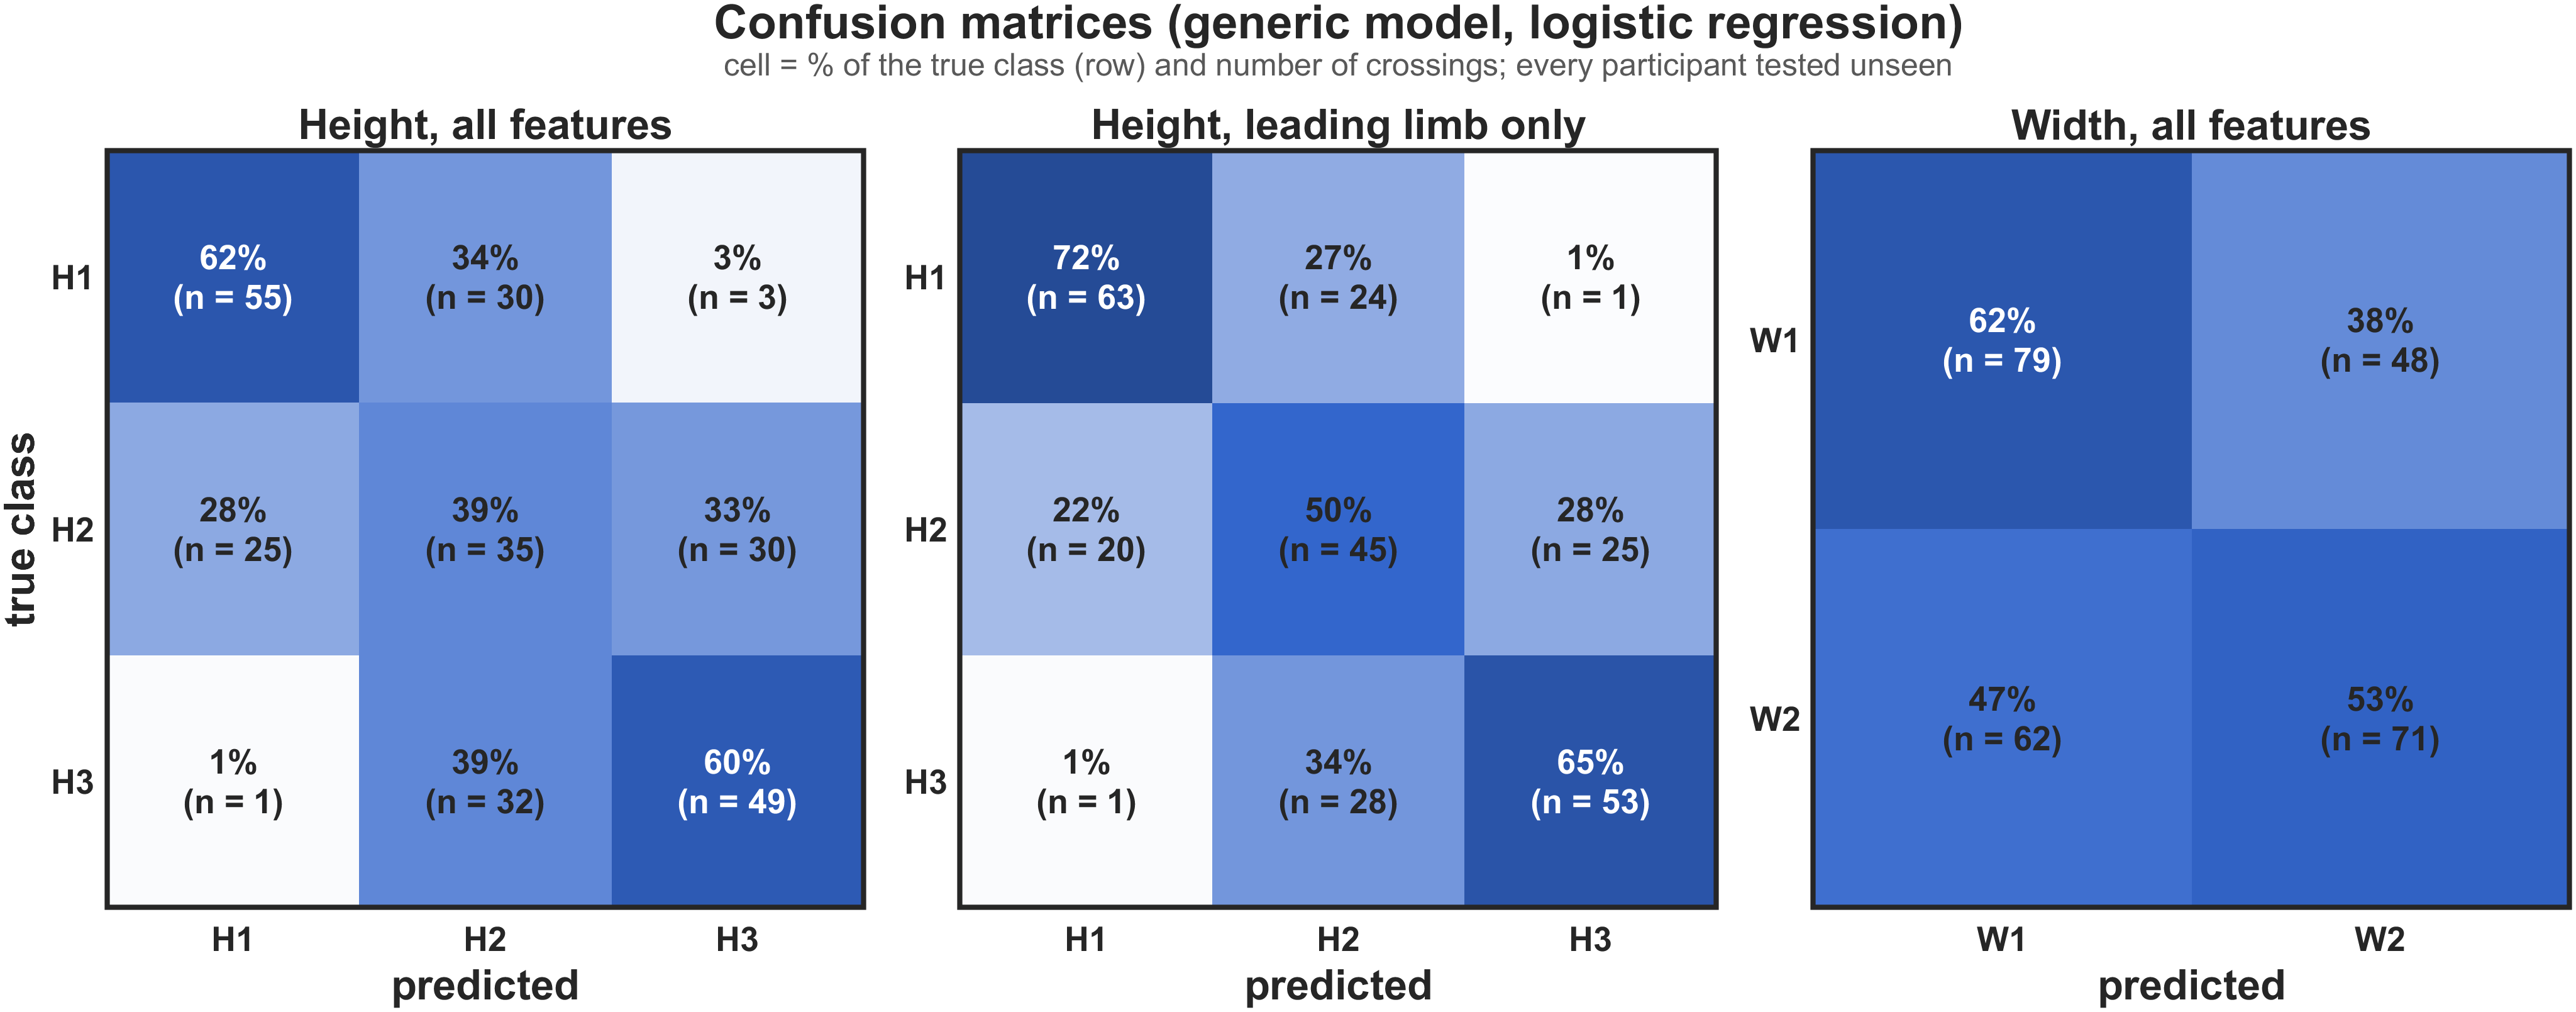
\includegraphics[width=\textwidth]{fig_confusion.png}
\caption{Confusion matrices of the generic model (logistic regression on level-walk-calibrated features): height from all features,
height from the leading limb only, and width. Cell = share of the true class (row) and number of crossings.}
\label{fig:confusion}
\end{figure}

\begin{figure}[htbp]
\centering
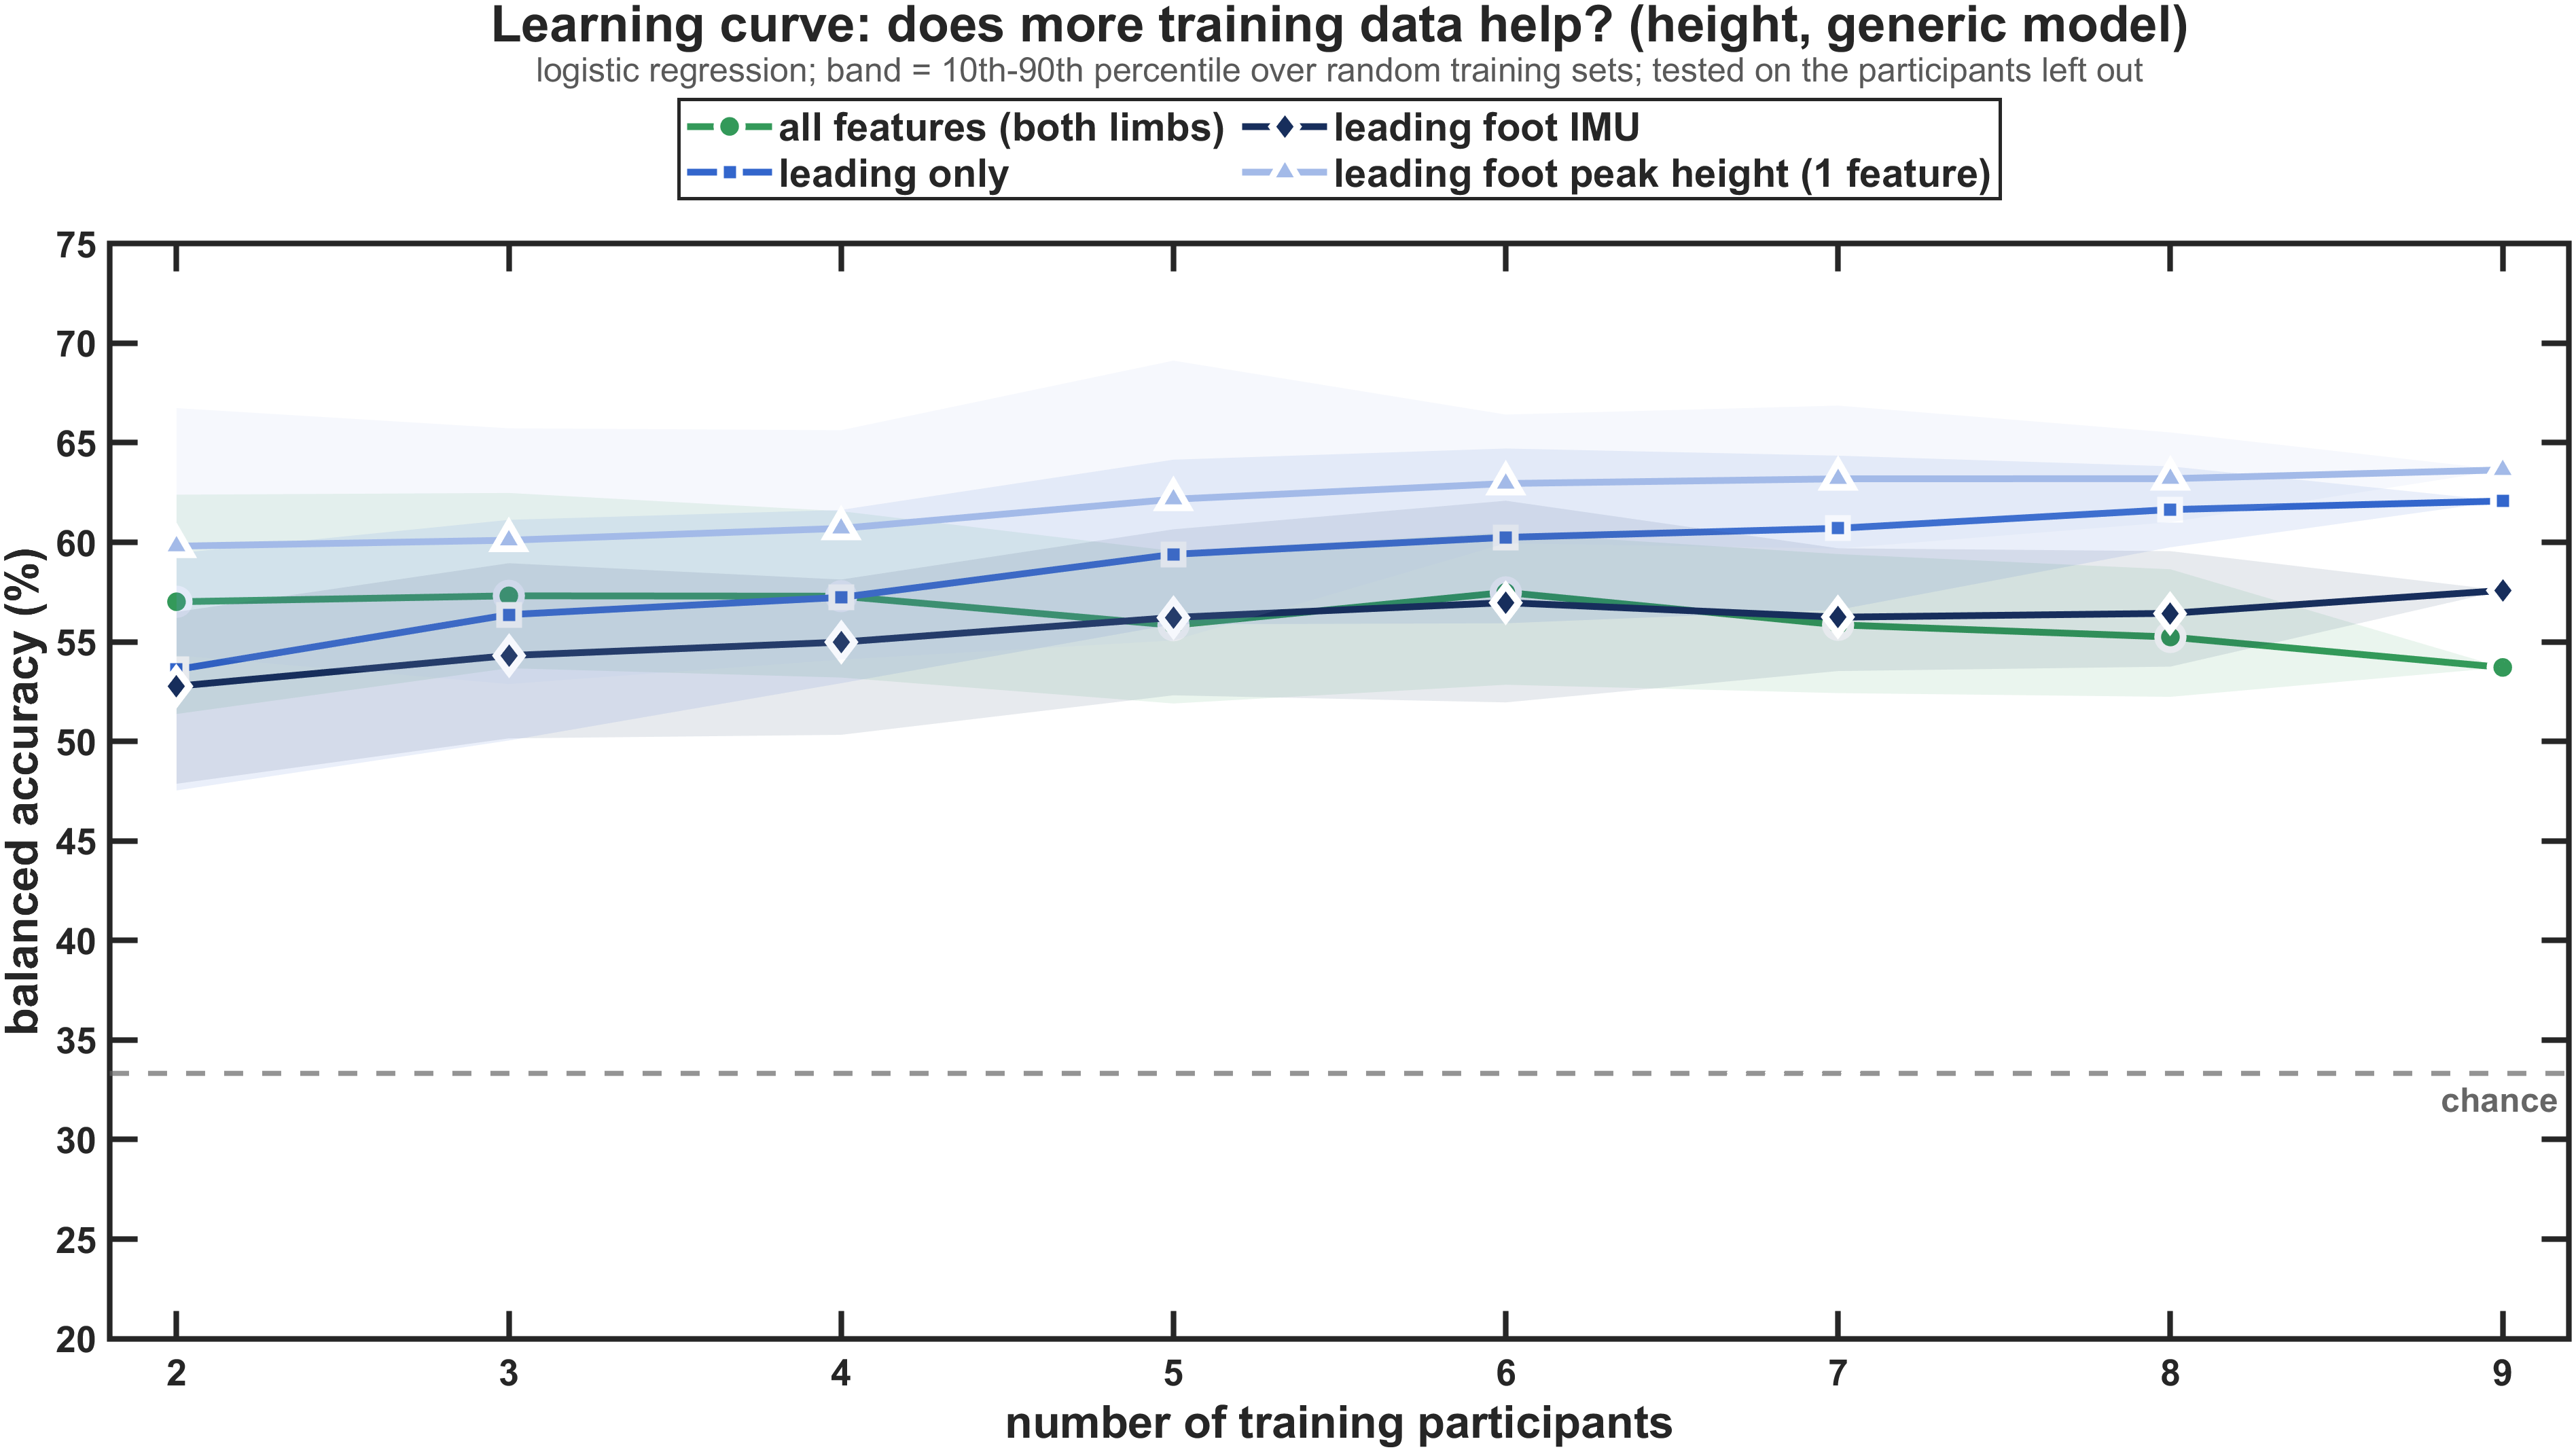
\includegraphics[width=\textwidth]{fig_learning_curve.png}
\caption{Learning curve of the generic model (height, logistic regression): each participant is predicted by a model trained on $n$
randomly chosen other participants (40 draws per $n$). Band = 10th--90th percentile over the draws; dashed = chance.}
\label{fig:learning}
\end{figure}

\subsubsection{Better inputs and models}

\paragraph{Clearance-shape features.} Thirteen numbers describing how long and how far the foot stays high
(Section~\ref{sec:features}) beat the 57 summary features in a generic model: 72.8\,\% vs 62.1\,\% with the leading limb and
logistic regression (permutation $p = 0.003$; Table~\ref{tab:inputs}). With person scaling they match the summary features
(89.7\,\% vs 90.4\,\% with the forest vote). The full swing curves do not add to the summary features.

\begin{table}[htbp]
\centering
\caption{Inputs compared: 57 summary features, 13 clearance-shape features, the swing curves and their combinations
(height; balanced accuracy, 95\,\% CI and the worst participant).}
\label{tab:inputs}
\begin{adjustbox}{max width=\textwidth}
{\footnotesize
\begin{tabular}{lrllrrr}
\toprule
\textbf{features} & \textbf{n feat (lead)} & \textbf{norm} & \textbf{model} & \textbf{lead} & \textbf{trail} & \textbf{fusion} \\
\midrule
summary & 57 & level & logreg & 62.1\% (55--70; worst 42\%) & 49.1\% (40--58; worst 27\%) & 56.1\% (46--66; worst 33\%) \\
summary & 57 & level & forest & 60.5\% (51--70; worst 31\%) & 58.8\% (47--71; worst 27\%) & 60.4\% (49--74; worst 27\%) \\
summary & 57 & self & logreg & 79.6\% (73--86; worst 57\%) & 78.0\% (67--87; worst 42\%) & 80.8\% (74--87; worst 65\%) \\
summary & 57 & self & forest & 88.4\% (83--93; worst 70\%) & 86.5\% (79--92; worst 62\%) & 90.4\% (85--95; worst 73\%) \\
shape & 13 & level & logreg & 72.8\% (65--80; worst 50\%) & 56.0\% (43--69; worst 27\%) & 63.7\% (51--77; worst 27\%) \\
shape & 13 & level & forest & 61.7\% (52--73; worst 38\%) & 53.6\% (42--66; worst 27\%) & 56.3\% (46--67; worst 27\%) \\
shape & 13 & self & logreg & 84.2\% (79--89; worst 72\%) & 75.1\% (68--81; worst 54\%) & 85.8\% (80--92; worst 65\%) \\
shape & 13 & self & forest & 86.1\% (82--91; worst 77\%) & 84.2\% (76--90; worst 58\%) & 89.7\% (86--93; worst 77\%) \\
curves & 66 & level & logreg & 60.6\% (52--68; worst 33\%) & 56.8\% (46--67; worst 27\%) & 57.9\% (47--70; worst 33\%) \\
curves & 66 & self & logreg & 75.0\% (68--81; worst 50\%) & 80.1\% (71--88; worst 50\%) & 82.3\% (75--90; worst 62\%) \\
summary + shape & 70 & level & logreg & 64.5\% (57--73; worst 42\%) & 50.6\% (41--60; worst 27\%) & 56.2\% (46--66; worst 33\%) \\
summary + shape & 70 & self & logreg & 83.4\% (77--89; worst 67\%) & 77.3\% (67--86; worst 42\%) & 83.0\% (77--89; worst 65\%) \\
summary + curves & 123 & level & logreg & 62.9\% (54--72; worst 37\%) & 53.1\% (42--64; worst 27\%) & 56.0\% (45--68; worst 33\%) \\
summary + curves & 123 & self & logreg & 80.8\% (77--85; worst 69\%) & 78.5\% (68--87; worst 42\%) & 82.3\% (75--89; worst 64\%) \\
\bottomrule
\end{tabular}
}
\end{adjustbox}

\end{table}

\paragraph{Models.} Random forests and boosted trees are the best single models with person scaling (88--90\,\%, soft vote);
the SVM and logistic regression are a few points lower (Table~\ref{tab:models}). A soft-vote ensemble of eight models reaches
91.5\,\%. The 1D convolutional network on the raw swing curves reaches 88.0\,\% with person scaling (Table~\ref{tab:cnn}) without
any hand-made feature, but no better than the forest on engineered features at this sample size.

\begin{table}[htbp]
\centering
\caption{Models compared with person scaling (height; balanced accuracy, 95\,\% CI, worst participant).}
\label{tab:models}
\begin{adjustbox}{max width=\textwidth}
{\footnotesize
\begin{tabular}{llrrr}
\toprule
\textbf{features} & \textbf{model} & \textbf{lead} & \textbf{trail} & \textbf{fusion} \\
\midrule
summary & logreg & 79.6\% (73--86; worst 57\%) & 78.0\% (67--87; worst 42\%) & 80.8\% (74--87; worst 65\%) \\
summary & forest & 88.4\% (83--93; worst 70\%) & 86.5\% (79--92; worst 62\%) & 90.4\% (85--95; worst 73\%) \\
summary & svm & 77.5\% (73--83; worst 67\%) & 80.0\% (72--87; worst 50\%) & 86.1\% (81--90; worst 69\%) \\
summary & boost & 87.3\% (81--92; worst 67\%) & 82.5\% (75--89; worst 54\%) & 88.4\% (83--94; worst 73\%) \\
shape & logreg & 84.2\% (79--89; worst 72\%) & 75.1\% (68--81; worst 54\%) & 85.8\% (80--92; worst 65\%) \\
shape & forest & 86.1\% (82--91; worst 77\%) & 84.2\% (76--90; worst 58\%) & 89.7\% (86--93; worst 77\%) \\
shape & svm & 81.5\% (76--87; worst 68\%) & 74.1\% (67--80; worst 54\%) & 86.9\% (82--92; worst 69\%) \\
shape & boost & 83.8\% (80--88; worst 73\%) & 86.2\% (81--90; worst 67\%) & 89.2\% (85--93; worst 80\%) \\
\bottomrule
\end{tabular}
}
\end{adjustbox}

\end{table}

\begin{table}[htbp]
\centering
\caption{1D convolutional network on the six swing curves of each limb (balanced accuracy).}
\label{tab:cnn}
\begin{adjustbox}{max width=\textwidth}
{\footnotesize
\begin{tabular}{llrrr}
\toprule
\textbf{normalization} & \textbf{target} & \textbf{lead} & \textbf{trail} & \textbf{fusion} \\
\midrule
level & height & 52.9\% & 53.1\% & 55.6\% \\
level & width & 52.3\% & 50.3\% & 50.7\% \\
self & height & 79.4\% & 82.6\% & 88.0\% \\
self & width & 50.0\% & 58.4\% & 56.5\% \\
\bottomrule
\end{tabular}
}
\end{adjustbox}

\end{table}

\paragraph{Honest selection.} Choosing the best setting by its test result is optimistic, so the choice was repeated inside each
training set (nested LOPO, Table~\ref{tab:nested}). Among generic settings the fair estimate is 69.4\,\% (58--80); among all 36
settings 91.5\,\% (86--97), with the person-scaled forest vote chosen in every fold (with summary + shape features in 9 of
10). Figure~\ref{fig:explore} summarises what each idea adds.

\begin{table}[htbp]
\centering
\caption{Nested selection of the setting (chosen inside each training set).}
\label{tab:nested}
\begin{adjustbox}{max width=\textwidth}
{\footnotesize
\begin{tabular}{lrp{3.6cm}p{6.6cm}}
\toprule
\textbf{candidate set} & \textbf{n settings} & \textbf{nested accuracy (95\% CI; worst participant)} & \textbf{settings chosen} \\
\midrule
generic & 18 & 69.4\% (58--80; worst 33\%) & shape, lead, logreg, level (9/10); summary, fusion, svm, level (1/10) \\
all & 36 & 91.5\% (86--97; worst 73\%) & summary + shape, fusion, forest, self (9/10); summary, fusion, forest, self (1/10) \\
\bottomrule
\end{tabular}
}
\end{adjustbox}

\end{table}

\begin{figure}[htbp]
\centering
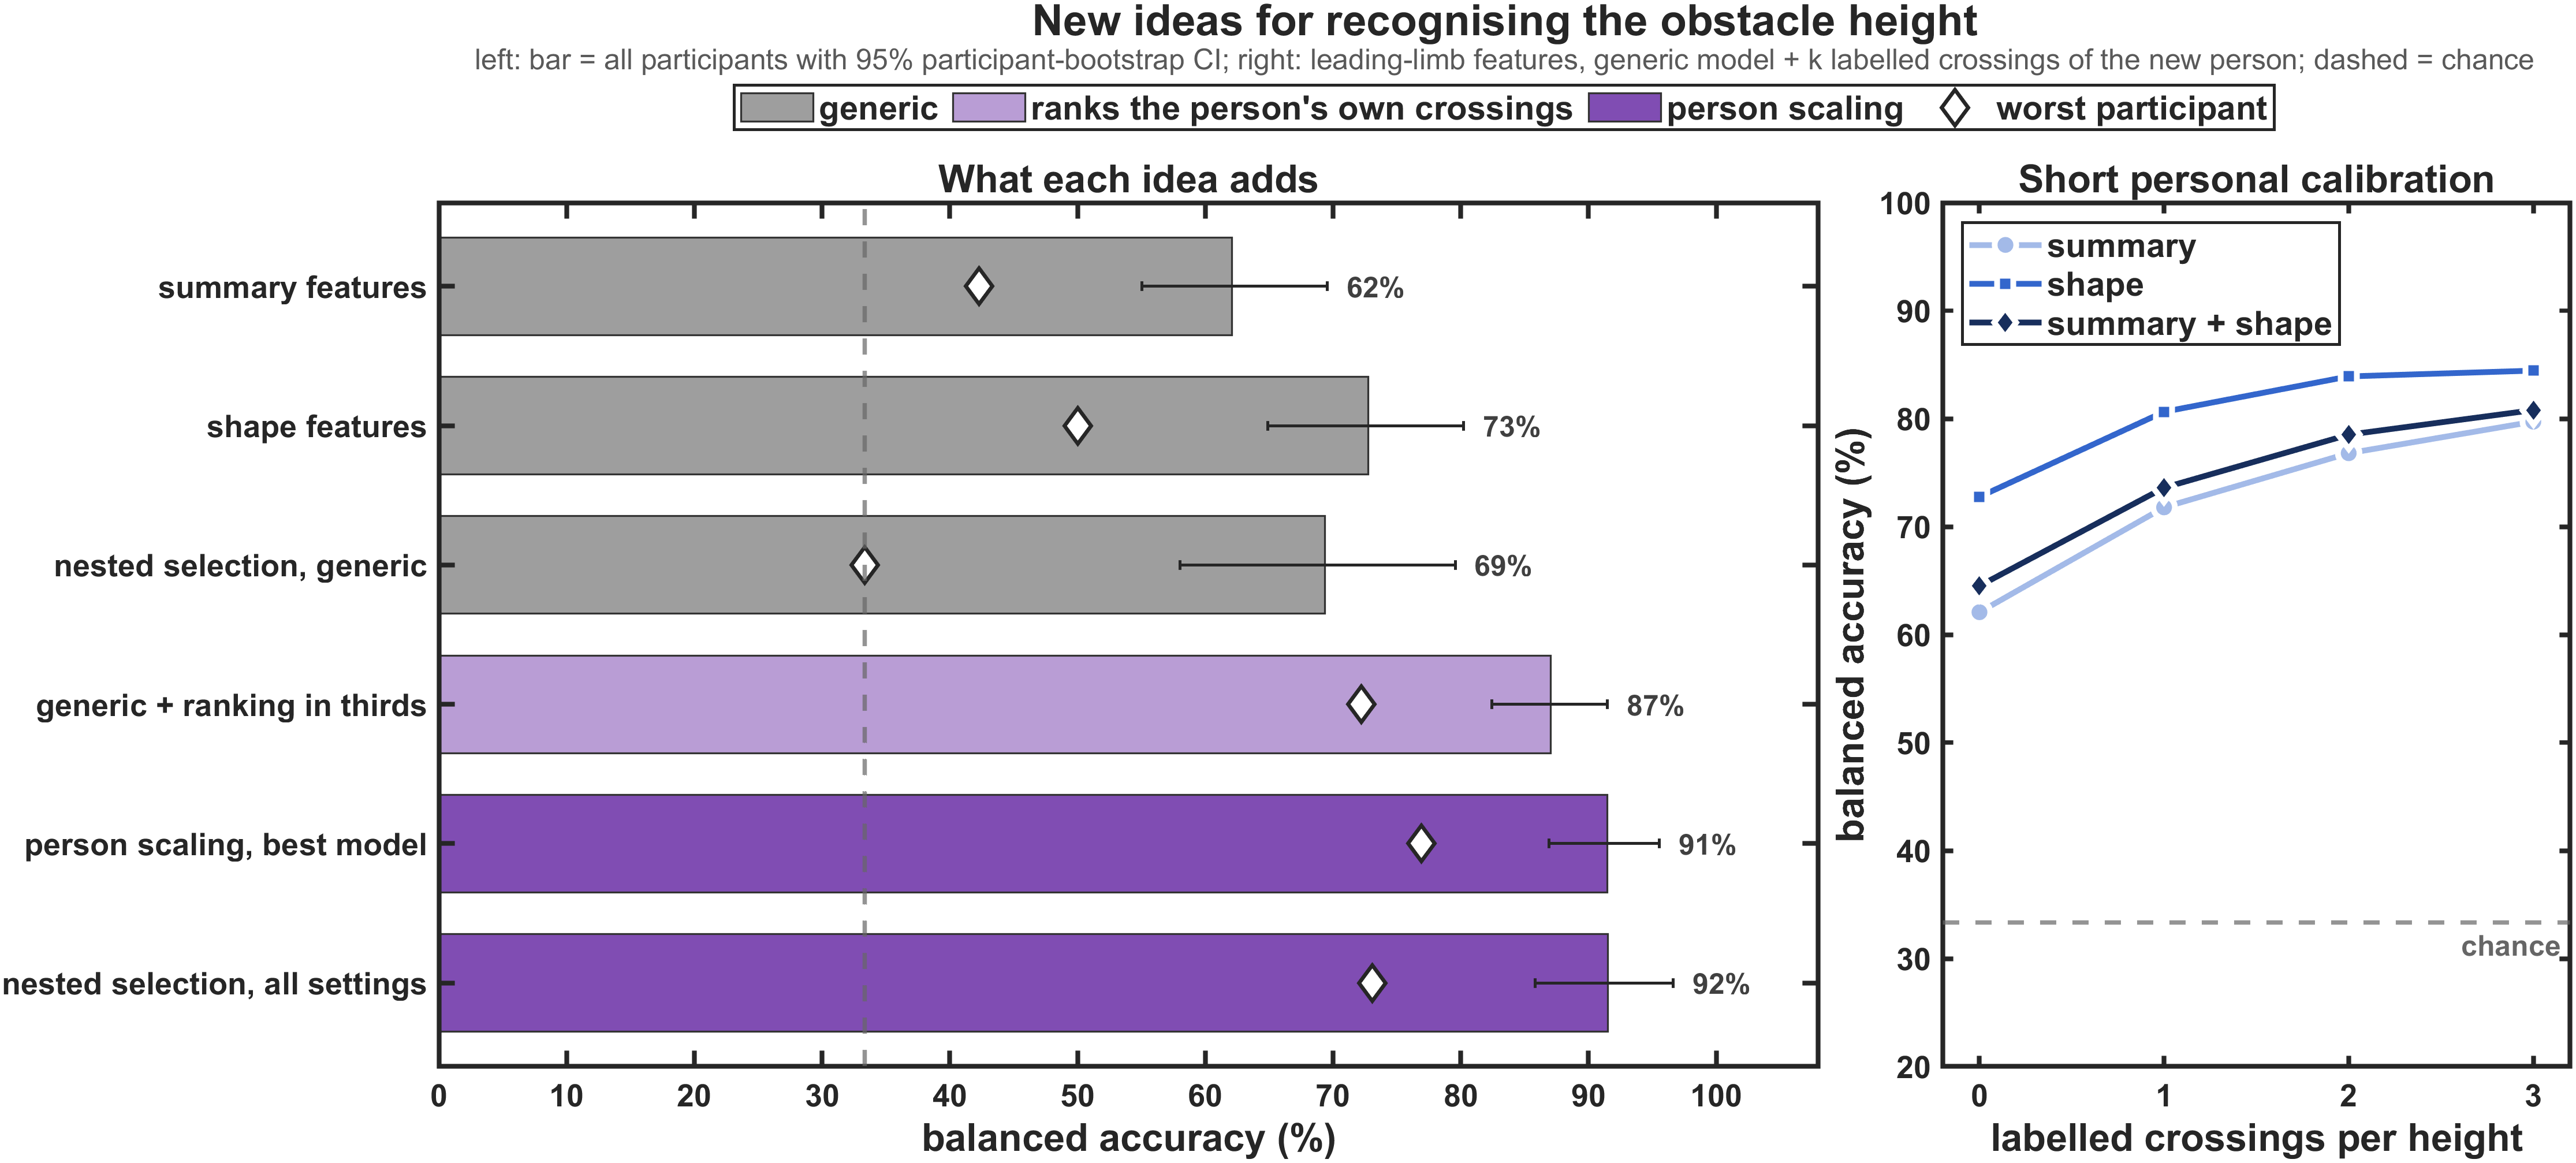
\includegraphics[width=\textwidth]{fig_explore.png}
\caption{Left: obstacle-height accuracy of the main ideas (bar = all participants with 95\,\% CI, diamond = worst participant;
grey = generic, light purple = ranks the person's own crossings, purple = person scaling). Right: generic model of the leading limb
plus a short personal calibration with $k$ labelled crossings per height.}
\label{fig:explore}
\end{figure}

\begin{table}[htbp]
\centering
\caption{What worked: summary of the model-improvement ideas (from \vn{ml_explore_matlab.md}).}
\label{tab:worked}
\begin{adjustbox}{max width=\textwidth}
{\footnotesize
\begin{tabular}{p{5.2cm}rrp{6.2cm}}
\toprule
\textbf{idea} & \textbf{before} & \textbf{after} & \textbf{comment} \\
\midrule
clearance-shape features, generic model (lead, level, logistic) & 62.1\% & \textbf{72.8\%} (p 0.003) & 13 features beat the 57 summary features without any person calibration \\
honest nested selection, generic settings only & 62.1\% & \textbf{69.4\%} (58--80) & best generic setting chosen fairly \\
+ ranking each person's crossings into thirds & 62.1\% & \textbf{87.0\%} & shape, fusion; assumes a mix of heights \\
1 labelled crossing per height from the new person & 71.8\% (summary) & \textbf{80.6\%} (shape) & 3 crossings of calibration \\
best single setting with self normalization & - & 90.4\% & summary, fusion, forest \\
best model / ensemble with self normalization & - & 91.5\% & ensemble (8 models), fusion, soft vote \\
honest nested selection, all settings & 89.3\% (Part 4.1) & \textbf{91.5\%} (86--97) & worst participant 73\% \\
self-training on the new person & 72.8\% (shape) & 54.0--67.1\% & did not help (the model reinforces its own errors) \\
width, best new idea & 64.3\% & 66.2\% & ratio + summary, fusion, logreg - width stays weak \\
\bottomrule
\end{tabular}
}
\end{adjustbox}

\end{table}

\subsubsection{Which segment and limb carries the information}

With person scaling (Table~\ref{tab:segments}), the foot is the best site: the foot angles alone give 88.1\,\% and the foot
trajectory 89.2\,\%. The thigh carries the leading limb's information (77.4\,\% leading, 44.2\,\% trailing) and the shank the
trailing limb's (78.2\,\% trailing, 49.8\,\% leading), matching where height appears in the signals (Figure~\ref{fig:map}). The
foot acceleration alone is weak.

Without person scaling (Figure~\ref{fig:featuresets}) every feature set predicts the height above its permutation null
($p \leq 0.037$), but the best set, the leading foot angles, reaches only 66.5\,\%. The limb pattern is the same as with person
scaling: the thigh and the foot angles carry more in the leading limb, the shank in the trailing limb. Width stays at 46--59\,\%,
around its null.

\begin{figure}[htbp]
\centering
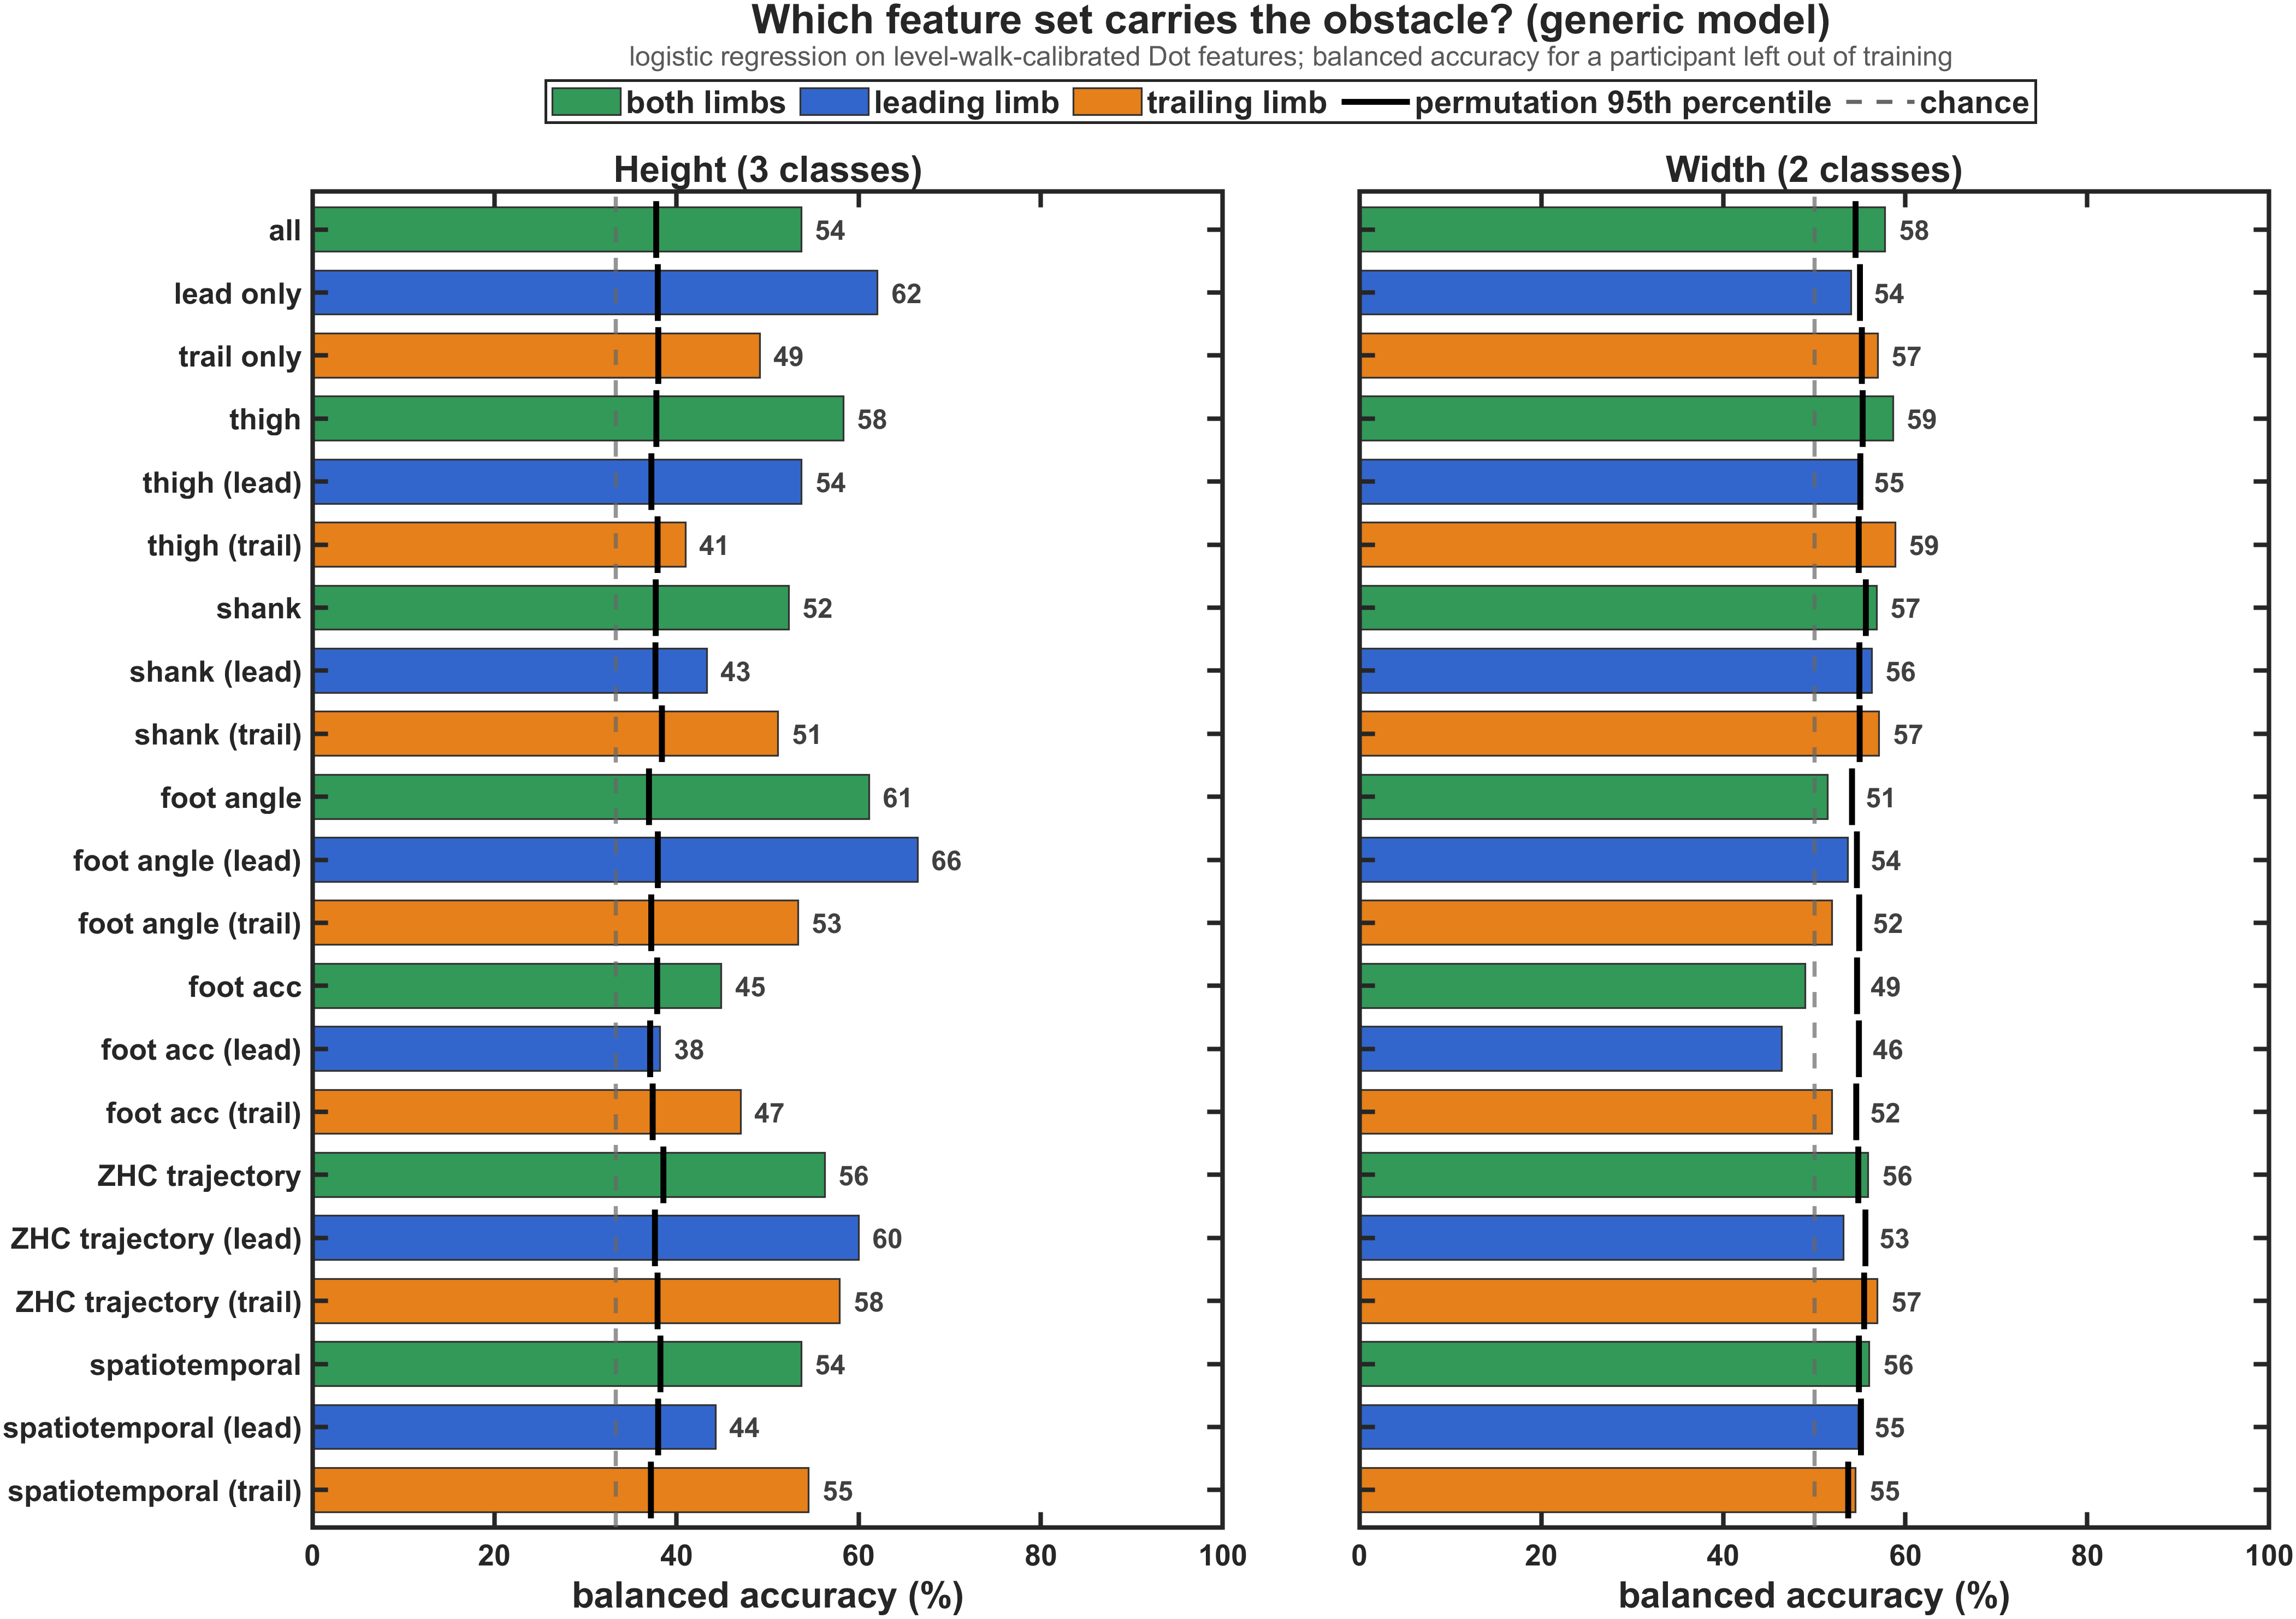
\includegraphics[width=\textwidth]{fig_feature_sets.png}
\caption{Generic model (logistic regression, level-walk calibration) for each Dot feature set: balanced accuracy for an unseen
participant, height (left) and width (right). Bar colour = limb of the set (blue = leading, orange = trailing, green = both);
black tick = 95th percentile of the permutation null (labels shuffled within participant); dashed = chance.}
\label{fig:featuresets}
\end{figure}

\begin{table}[htbp]
\centering
\caption{Height accuracy per segment and limb with person scaling (logistic regression and random forest).}
\label{tab:segments}
\begin{adjustbox}{max width=\textwidth}
{\footnotesize
\begin{tabular}{lrrr}
\toprule
\textbf{features} & \textbf{n feat} & \textbf{logistic (C = 0.1)} & \textbf{random forest} \\
\midrule
lead only & 57 & 79.6\% (73--86) & 88.4\% (83--93) \\
trail only & 52 & 78.0\% (67--87) & 86.5\% (79--92) \\
thigh & 24 & 73.4\% (65--80) & 77.6\% (66--87) \\
thigh (lead) & 12 & 78.0\% (68--87) & 77.4\% (67--85) \\
thigh (trail) & 12 & 47.4\% (39--55) & 44.2\% (35--53) \\
shank & 24 & 69.6\% (62--76) & 79.4\% (69--88) \\
shank (lead) & 12 & 45.2\% (39--52) & 49.8\% (41--56) \\
shank (trail) & 12 & 72.7\% (65--79) & 78.2\% (68--86) \\
foot angle & 26 & 84.7\% (77--91) & 88.1\% (83--93) \\
foot angle (lead) & 13 & 83.9\% (79--89) & 88.1\% (84--92) \\
foot angle (trail) & 13 & 75.5\% (67--83) & 83.4\% (75--90) \\
foot acc & 6 & 51.4\% (43--61) & 58.0\% (49--67) \\
foot acc (lead) & 3 & 34.1\% (29--39) & 36.9\% (30--44) \\
foot acc (trail) & 3 & 52.3\% (43--61) & 54.0\% (46--62) \\
ZHC trajectory & 22 & 88.4\% (83--93) & 89.2\% (83--94) \\
ZHC trajectory (lead) & 11 & 81.2\% (78--85) & 84.9\% (80--89) \\
ZHC trajectory (trail) & 11 & 82.3\% (74--89) & 84.5\% (75--92) \\
spatiotemporal & 10 & 68.7\% (59--77) & 71.6\% (63--80) \\
spatiotemporal (lead) & 7 & 54.3\% (47--62) & 55.4\% (50--62) \\
spatiotemporal (trail) & 2 & 68.4\% (60--77) & 66.5\% (59--74) \\
\bottomrule
\end{tabular}
}
\end{adjustbox}

\end{table}

\subsubsection{When the height is known}

Using only the leading limb's data available up to a given moment of its swing (Table~\ref{tab:timing},
Figure~\ref{fig:settings}), the person-scaled forest already reaches 52\,\% at the leading toe-off, about 80\,\% by its apex
(50\,\% of the swing, a median 458\,ms before the trailing toe leaves the floor) and 88.5\,\% at 70\,\% of the swing (355\,ms
before). The generic model stays at 41--65\,\%. With logistic regression (Figure~\ref{fig:cueing}) the generic model rises
from 42\,\% at the leading toe-off to about 60\,\% by the leading foot apex and stays there.

\begin{table}[htbp]
\centering
\caption{Height from the leading limb's data up to $x$\,\% of its swing, with the median time left before the trailing toe
lift-off (camera).}
\label{tab:timing}
\begin{adjustbox}{max width=\textwidth}
{\footnotesize
\begin{tabular}{lrrrrr}
\toprule
\textbf{data up to} & \textbf{ms before the trailing lift-off} & \textbf{level, logistic} & \textbf{level, forest} & \textbf{self, logistic} & \textbf{self, forest} \\
\midrule
0\% & 733 & 42.0\% & 41.2\% & 46.7\% & 52.1\% \\
10\% & 682 & 50.0\% & 48.0\% & 58.3\% & 63.8\% \\
20\% & 630 & 54.2\% & 53.5\% & 63.8\% & 69.7\% \\
30\% & 573 & 51.8\% & 55.8\% & 65.0\% & 73.8\% \\
40\% & 517 & 58.3\% & 61.2\% & 68.5\% & 79.0\% \\
50\% & 458 & 59.9\% & 62.8\% & 73.5\% & 80.5\% \\
60\% & 410 & 61.5\% & 64.6\% & 77.4\% & 80.4\% \\
70\% & 355 & 58.7\% & 64.0\% & 83.9\% & 88.5\% \\
80\% & 303 & 60.2\% & 62.4\% & 82.0\% & 86.5\% \\
90\% & 248 & 58.1\% & 55.6\% & 81.4\% & 86.8\% \\
100\% & 200 & 59.4\% & 57.0\% & 80.7\% & 85.8\% \\
\bottomrule
\end{tabular}
}
\end{adjustbox}

\end{table}

\begin{figure}[htbp]
\centering
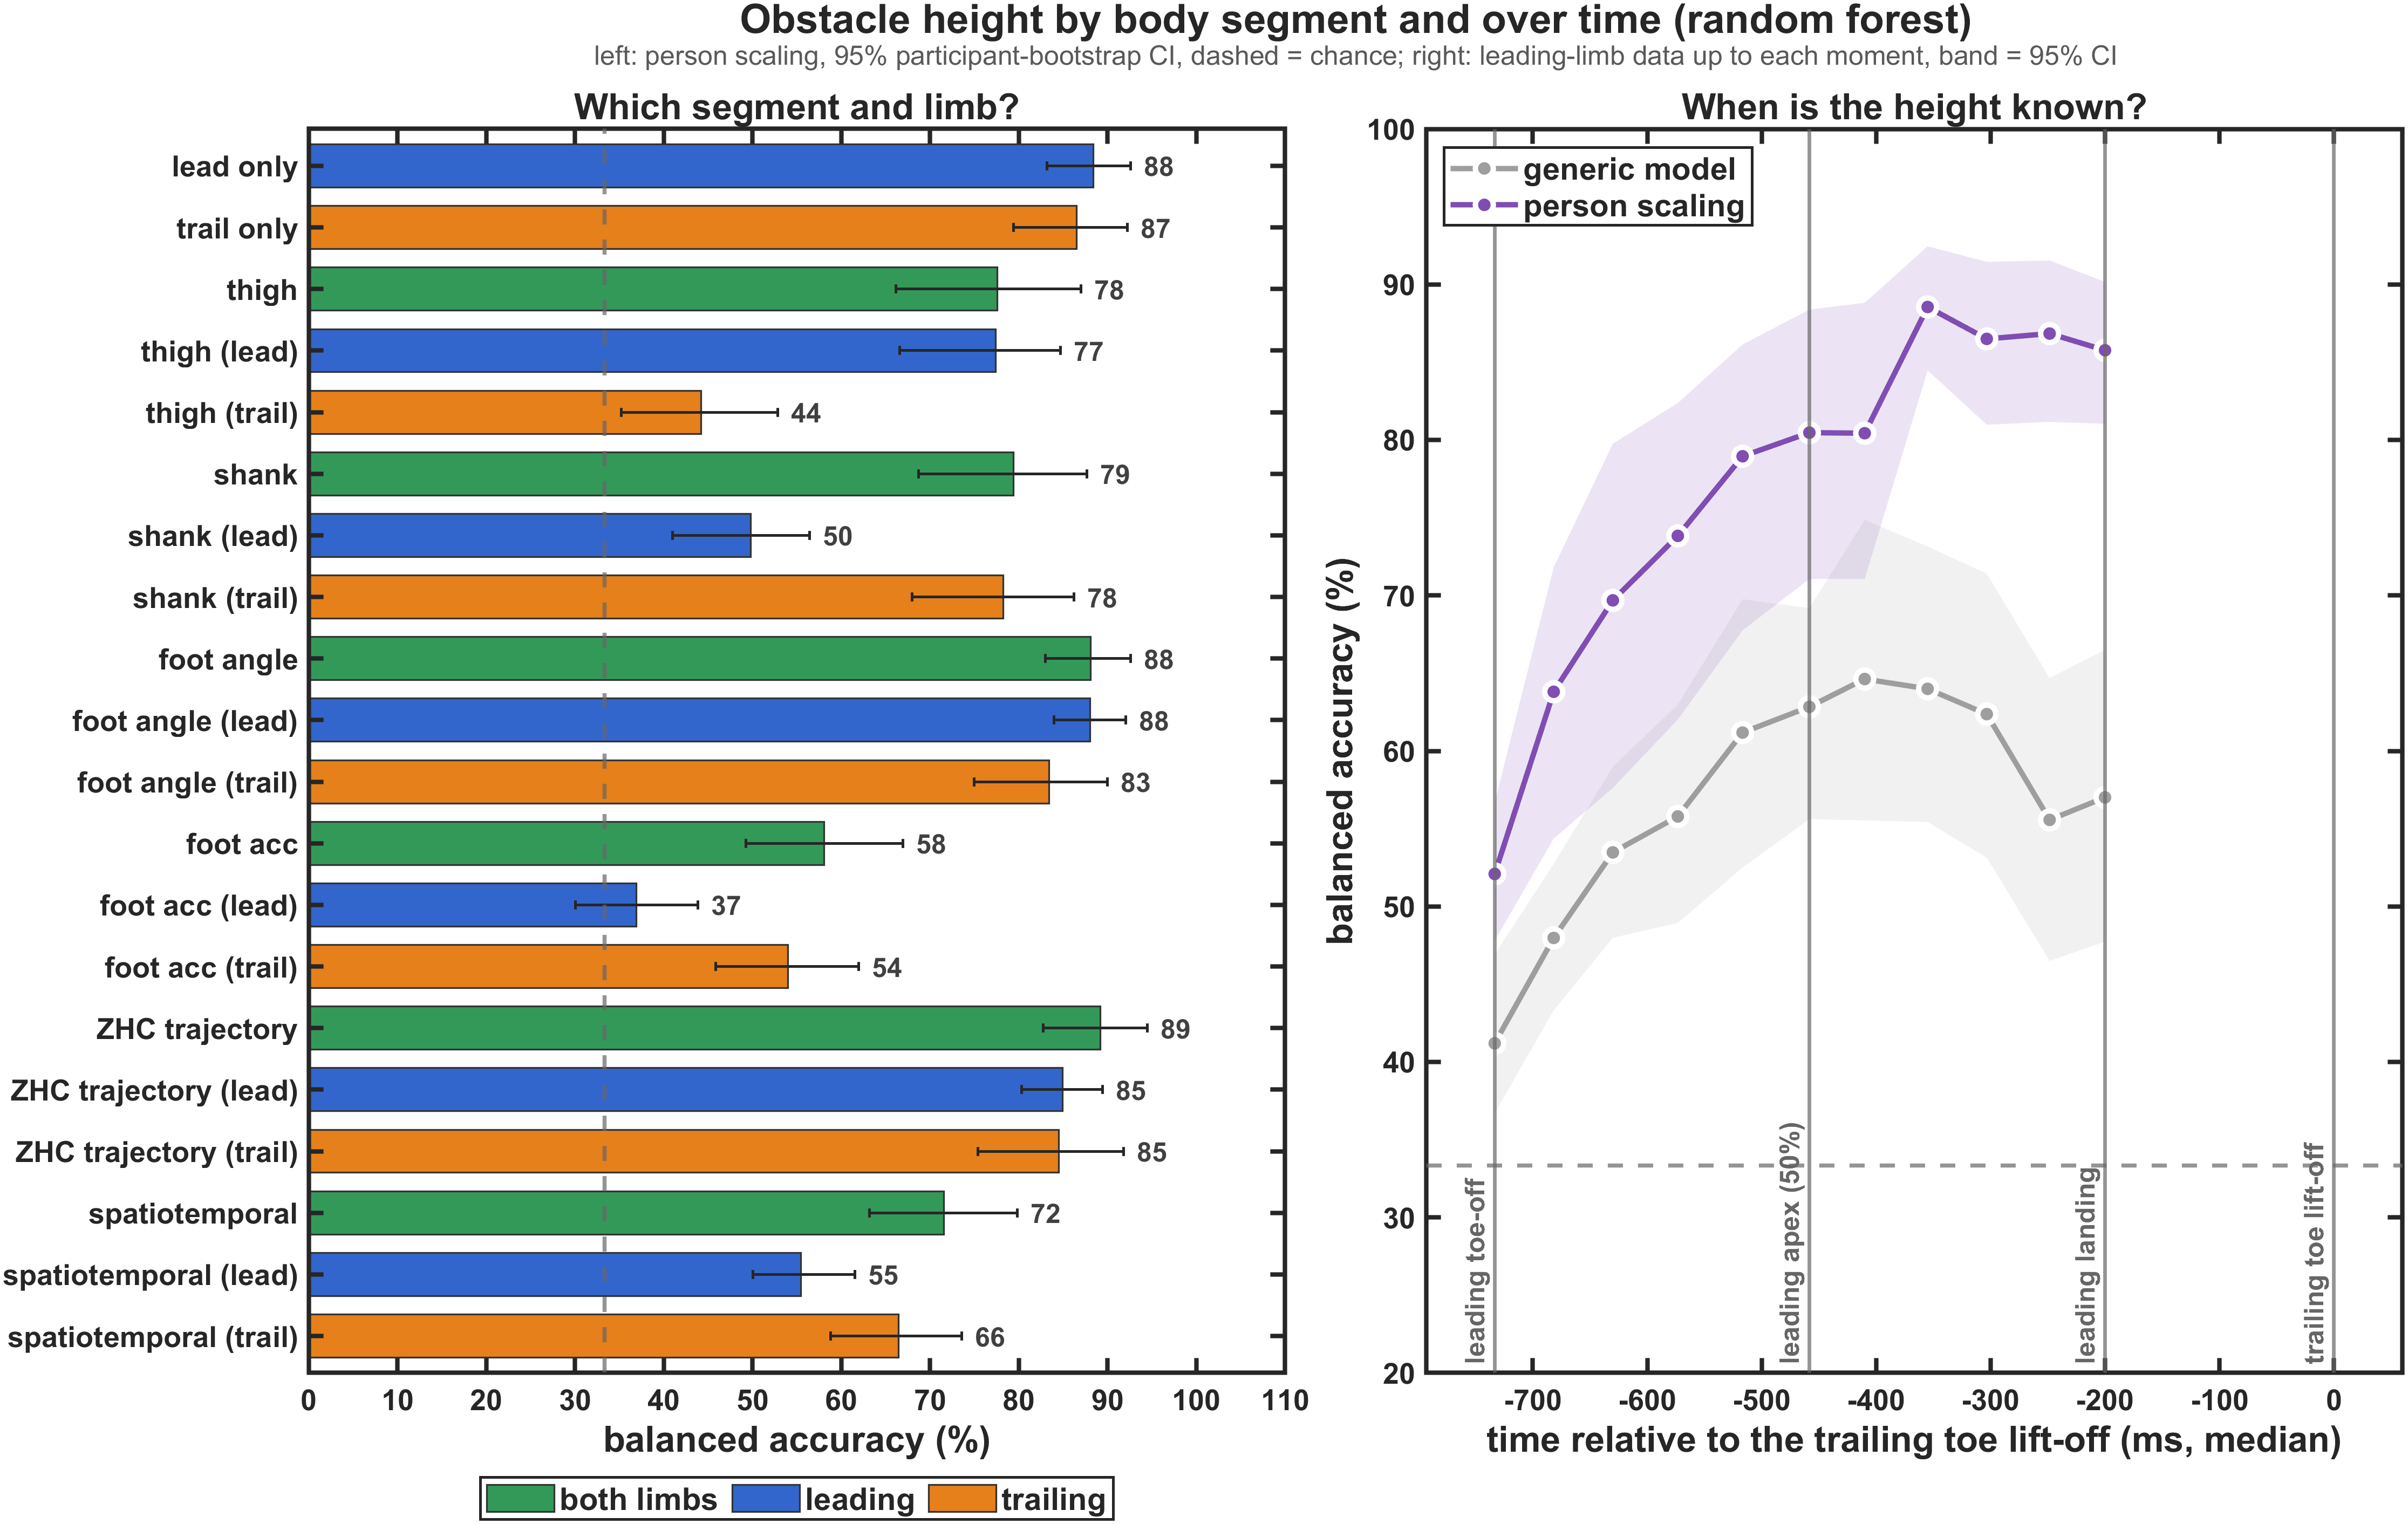
\includegraphics[width=\textwidth]{fig_settings.png}
\caption{Left: height accuracy by segment and limb with person scaling (random forest; blue = leading, orange = trailing,
green = both limbs; 95\,\% CI). Right: height from the leading-limb data available so far, generic (grey) vs person scaling (purple),
against the median time relative to the trailing toe lift-off (band = 95\,\% CI).}
\label{fig:settings}
\end{figure}

\begin{figure}[htbp]
\centering
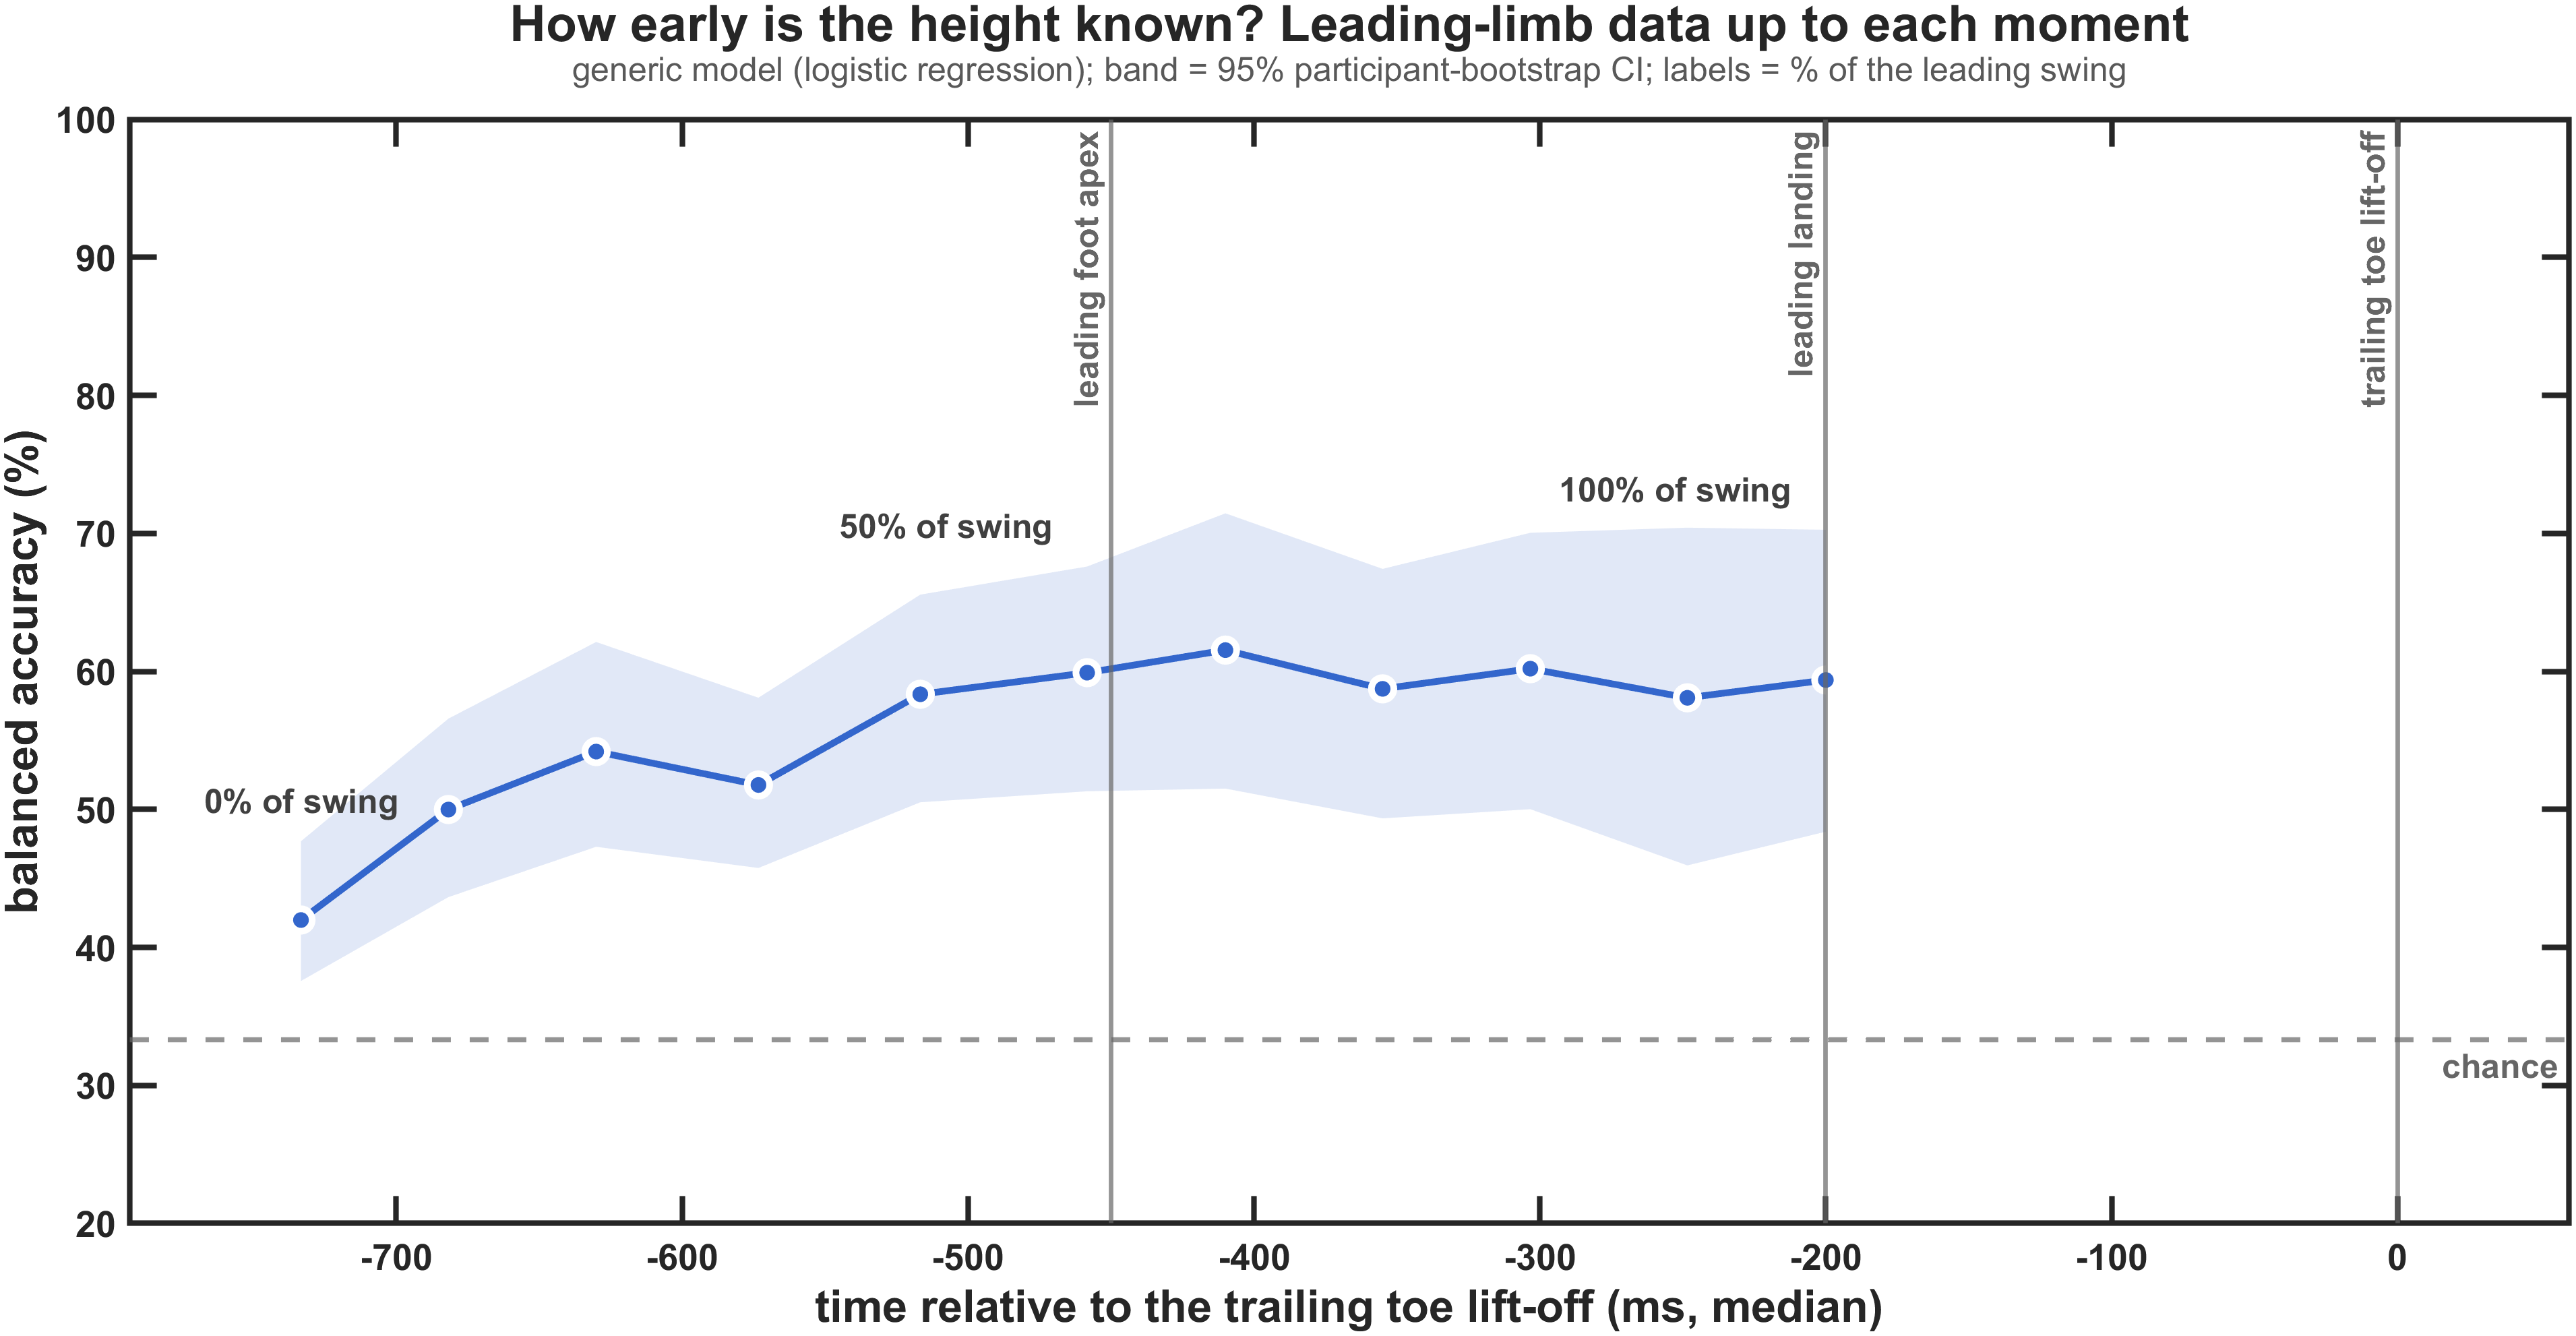
\includegraphics[width=\textwidth]{fig_cueing_time.png}
\caption{Generic model (logistic regression) using the leading-limb data available up to each moment of its swing (labels = \% of the
swing), against the median time relative to the trailing toe lift-off. Band = 95\,\% participant-bootstrap CI; vertical lines =
median leading foot apex, leading landing and trailing toe lift-off; dashed = chance.}
\label{fig:cueing}
\end{figure}

\subsubsection{Height as a number}

Regressing the obstacle height in centimetres (Table~\ref{tab:cm}), the person-scaled forest vote has a mean absolute error of
2.39\,cm ($r = 0.91$); rounding to the nearest of the person's three nominal heights gives 84.8\,\%. Neighbouring heights are
8.3--10.6\,cm apart, so the typical error is about a quarter of a step.

\begin{table}[htbp]
\centering
\caption{Obstacle height in centimetres (regression), and the class nearest to the estimate.}
\label{tab:cm}
\begin{adjustbox}{max width=\textwidth}
{\footnotesize
\begin{tabular}{llrrr}
\toprule
\textbf{inputs} & \textbf{model} & \textbf{MAE (cm)} & \textbf{r} & \textbf{class from cm (bal. acc)} \\
\midrule
lead, level & ridge & 5.19 & 0.69 & 63.5\% \\
lead, level & forest & 4.19 & 0.72 & 61.7\% \\
lead, self & ridge & 3.51 & 0.79 & 76.8\% \\
lead, self & forest & 2.42 & 0.88 & 83.3\% \\
lead + trail vote, self & ridge & 3.32 & 0.84 & 76.7\% \\
lead + trail vote, self & forest & 2.39 & 0.91 & 84.8\% \\
\bottomrule
\end{tabular}
}
\end{adjustbox}

\end{table}

\subsubsection{Per participant, and two easier tasks}

With person scaling the accuracy is 83--100\,\% for nine participants and 73\,\% for participant 108
(Table~\ref{tab:perparticipant}; the reason is shown in Section~\ref{sec:res-device}). Two related tasks are solved almost
perfectly by the Dot: telling the leading from the trailing limb's swing (100\,\%, Table~\ref{tab:leadtrail}) and telling an
obstacle crossing from a level-walk stride (100\,\%, Table~\ref{tab:obslevel}).

The generic model varies much more between people (Figure~\ref{fig:participants}): 31--74\,\% with all features and 42--85\,\% with
the leading limb only. Participant 108 reaches 85\,\% from the leading limb alone but only 38\,\% with all features and 31\,\% with
the trailing limb, whose lift is the least consistent in the group (Section~\ref{sec:res-device}).

\begin{figure}[htbp]
\centering
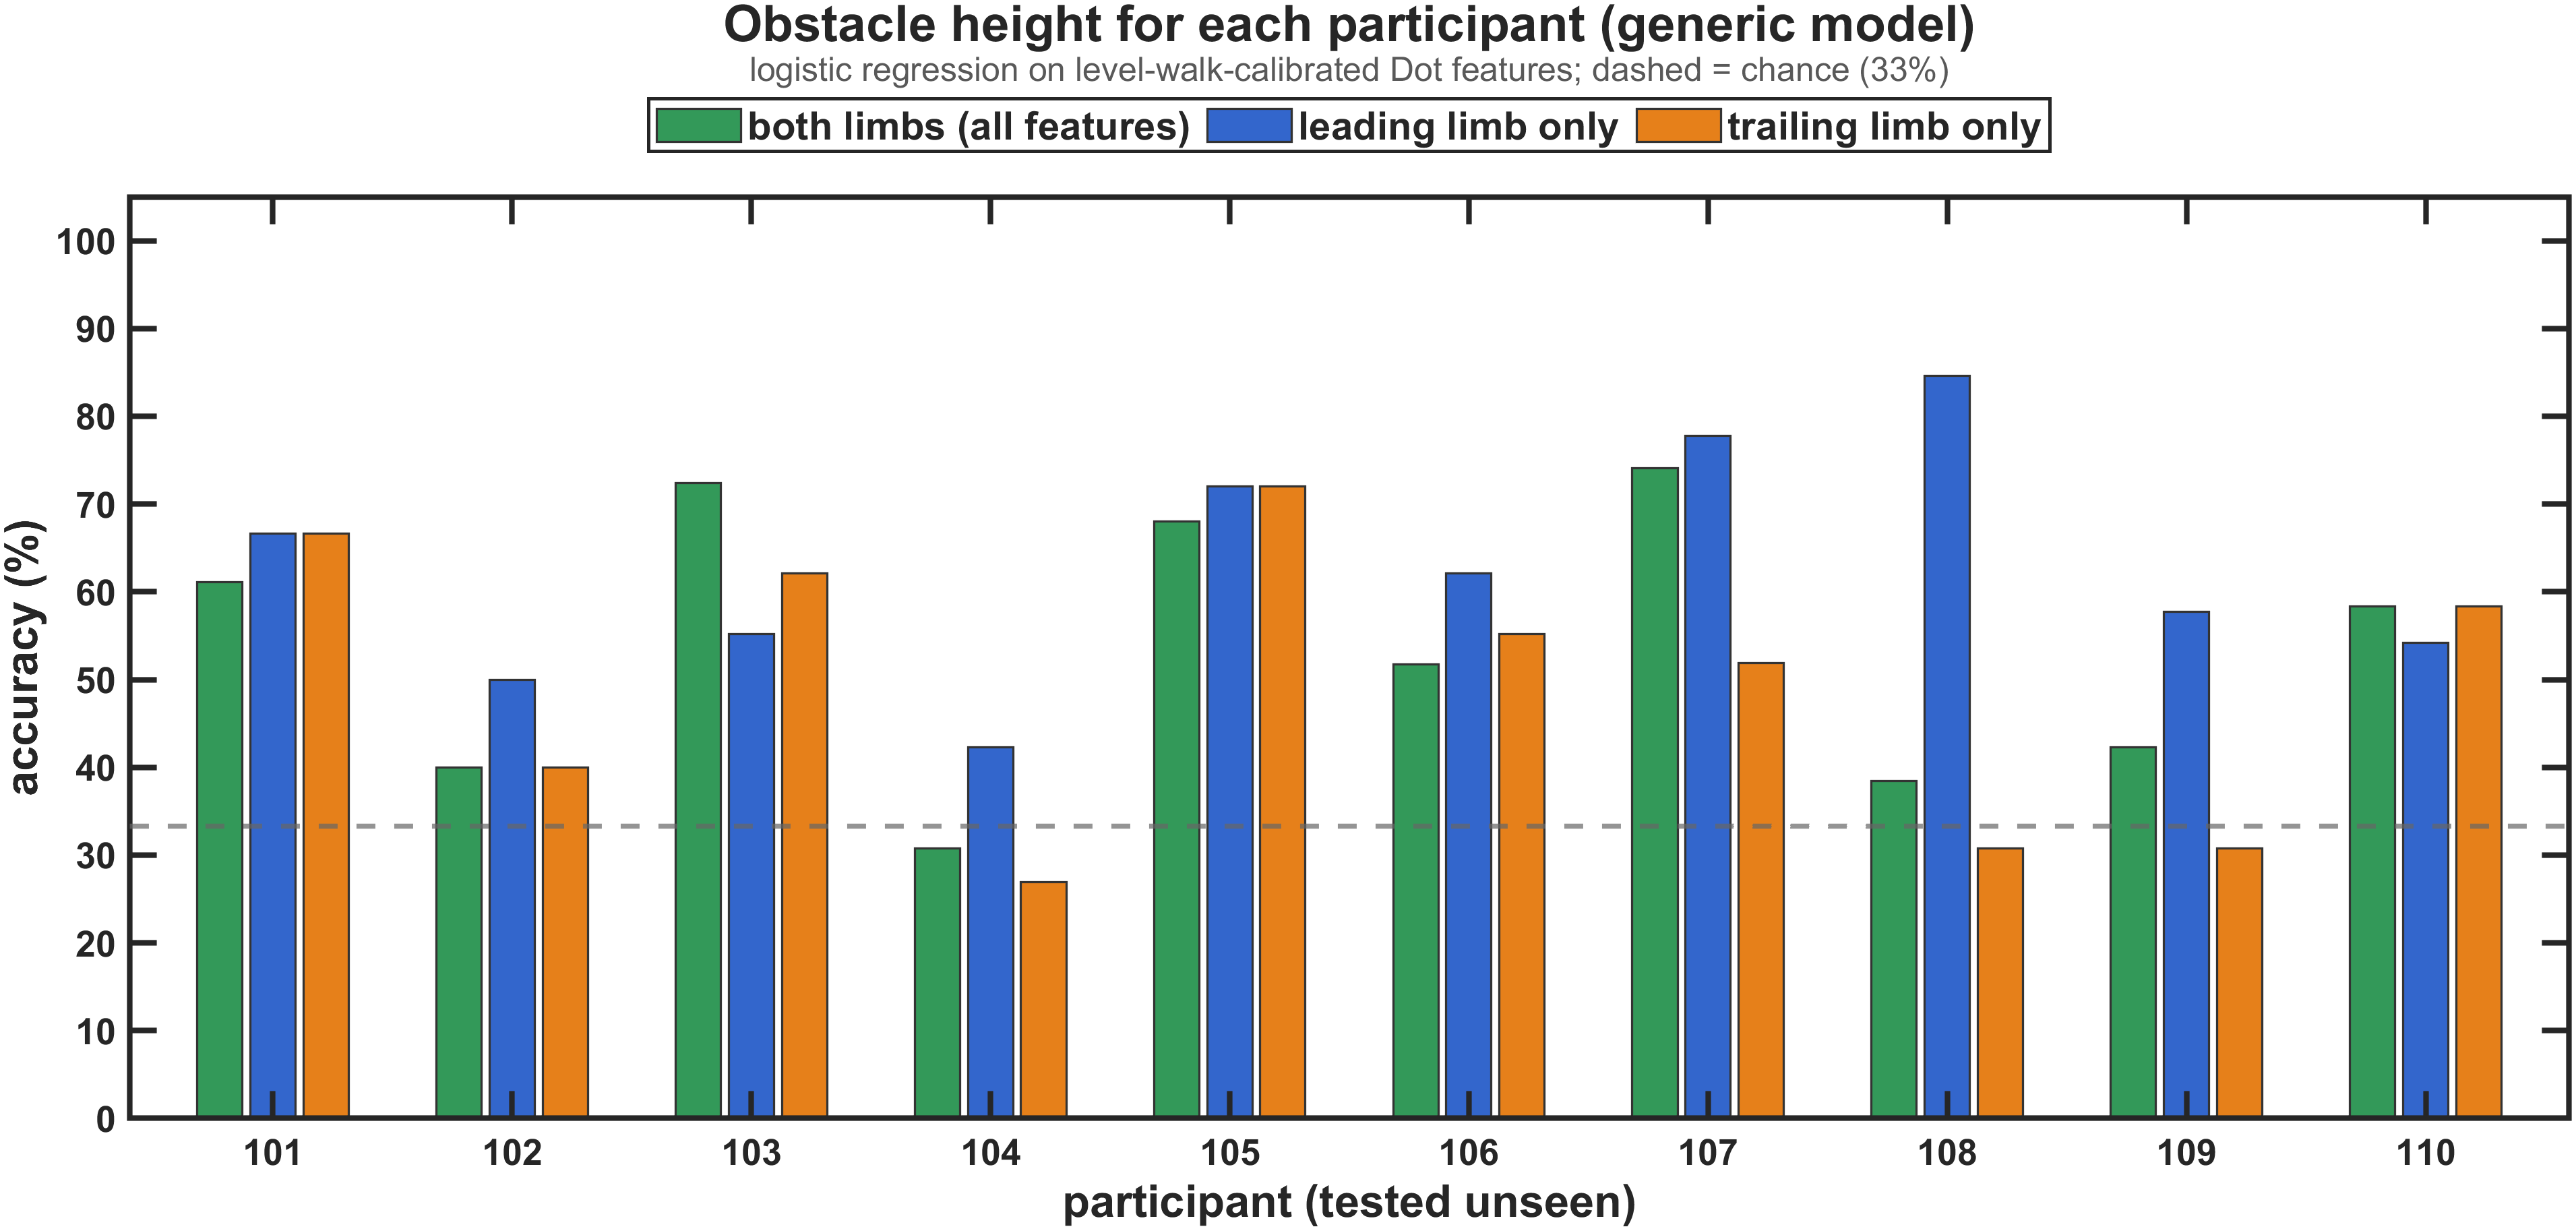
\includegraphics[width=\textwidth]{fig_participants.png}
\caption{Generic model (logistic regression) for each participant when left out of training: all features (green), the leading limb
only (blue) and the trailing limb only (orange). Dashed = chance.}
\label{fig:participants}
\end{figure}

\begin{table}[htbp]
\centering
\caption{Height accuracy for each left-out participant.}
\label{tab:perparticipant}
\begin{adjustbox}{max width=\textwidth}
{\footnotesize
\begin{tabular}{lrrrrrrrrrrr}
\toprule
\textbf{setting} & \textbf{101} & \textbf{102} & \textbf{103} & \textbf{104} & \textbf{105} & \textbf{106} & \textbf{107} & \textbf{108} & \textbf{109} & \textbf{110} & \textbf{overall} \\
\midrule
level, logreg C=0.1, lead & 67\% & 50\% & 55\% & 42\% & 72\% & 62\% & 78\% & 85\% & 58\% & 54\% & 62.1\% \\
self, logreg C=0.1, lead & 94\% & 57\% & 90\% & 92\% & 84\% & 83\% & 70\% & 73\% & 77\% & 83\% & 79.6\% \\
self, forest, lead & 94\% & 70\% & 97\% & 92\% & 92\% & 83\% & 89\% & 88\% & 92\% & 92\% & 88.4\% \\
self, forest, fusion & 94\% & 83\% & 97\% & 96\% & 100\% & 93\% & 85\% & 73\% & 88\% & 96\% & 90.4\% \\
\bottomrule
\end{tabular}
}
\end{adjustbox}

\end{table}

\begin{table}[htbp]
\centering
\begin{minipage}{0.48\textwidth}
\centering
\caption{Leading or trailing limb, from one swing.}
\label{tab:leadtrail}
\begin{adjustbox}{max width=\textwidth}
{\footnotesize
\begin{tabular}{llrrr}
\toprule
\textbf{norm} & \textbf{model} & \textbf{bal. acc} & \textbf{95\% CI} & \textbf{perm p} \\
\midrule
raw & logreg & 100.0\% & 100--100 & 0.003 \\
raw & forest & 100.0\% & 100--100 & - \\
level & logreg & 100.0\% & 100--100 & 0.003 \\
level & forest & 100.0\% & 100--100 & - \\
self & logreg & 100.0\% & 100--100 & 0.003 \\
self & forest & 100.0\% & 100--100 & - \\
\bottomrule
\end{tabular}
}
\end{adjustbox}

\end{minipage}\hfill
\begin{minipage}{0.48\textwidth}
\centering
\caption{Obstacle crossing or level-walk stride.}
\label{tab:obslevel}
\begin{adjustbox}{max width=\textwidth}
{\footnotesize
\begin{tabular}{llrrr}
\toprule
\textbf{norm} & \textbf{model} & \textbf{lead} & \textbf{trail} & \textbf{fusion} \\
\midrule
raw & logreg & 100.0\% (100--100) & 97.1\% (92--100) & 100.0\% (100--100) \\
raw & forest & 99.8\% (99--100) & 99.8\% (99--100) & 100.0\% (100--100) \\
self & logreg & 94.9\% (84--100) & 100.0\% (100--100) & 100.0\% (100--100) \\
self & forest & 100.0\% (100--100) & 99.8\% (99--100) & 100.0\% (100--100) \\
\bottomrule
\end{tabular}
}
\end{adjustbox}

\end{minipage}
\end{table}

\subsubsection{Generalisation to obstacles not seen in training}
\label{sec:res-general}

\paragraph{Unseen heights.} Real obstacles have arbitrary heights, so the regression was also trained with one height level removed
from the training data (Table~\ref{tab:unseenheight}). Interpolation works: a ridge model that never saw the middle height (H2)
estimates it with a 3.1\,cm mean absolute error and puts 79\,\% of those crossings at the right level (88\,\% when trained on all
heights). Extrapolation is biased toward the trained range: an unseen lowest or highest height is over- or under-estimated by about
half a step (+4.0 and $-5.7$\,cm). The random forest cannot extrapolate at all (an unseen H1 or H3 is off by a full step), and the
generic models are worse throughout. A device for obstacles of any height should therefore be trained on obstacles that span the
heights it will meet, with a model that scales linearly with height.

\begin{table}[htbp]
\centering
\caption{Height in cm when a height level is missing from training (person scaling). Cells: mean absolute error in cm (mean signed
error, + = too high); ``right level'' = the estimate is closest to the person's true nominal height.}
\label{tab:unseenheight}
\begin{adjustbox}{max width=\textwidth}
{\scriptsize
\begin{tabular}{llrrrr}
\toprule
\textbf{model} & \textbf{training} & \textbf{H1 tested} & \textbf{H2 tested} & \textbf{H3 tested} & \textbf{all} \\
\midrule
ridge & all heights trained & 3.0 (+1.4); right level 81\% & 2.6 (+1.0); right level 88\% & 3.8 ($-$2.3); right level 77\% & 3.1 (+0.1); right level 82\% \\
ridge & this height left out & 4.7 (+4.0); right level 50\% & 3.1 (+1.8); right level 79\% & 6.0 ($-$5.7); right level 37\% & 4.6 (+0.2); right level 56\% \\
forest & all heights trained & 1.4 (+1.2); right level 91\% & 2.7 (+1.1); right level 86\% & 3.1 ($-$2.6); right level 79\% & 2.4 ($-$0.0); right level 85\% \\
forest & this height left out & 10.8 (+10.8); right level 0\% & 5.3 (+3.1); right level 42\% & 9.8 ($-$9.8); right level 0\% & 8.6 (+1.6); right level 15\% \\
\bottomrule
\end{tabular}
}
\end{adjustbox}

\end{table}

\paragraph{Unseen width.} Height recognition trained on crossings of one width only and tested on the other width loses about
6.5 points compared with training on the same width with the same amount of data (86.2\,\% vs 92.7\,\%, Table~\ref{tab:unseenwidth}):
although width itself is barely recognisable, the obstacle depth slightly changes how the height shows in the foot motion, so
training data should include obstacles of different depths.

\begin{table}[htbp]
\centering
\caption{Height recognition tested on one width, trained on the same width, the other width only, or both (two foot IMUs, person
scaling, forest vote).}
\label{tab:unseenwidth}
\begin{adjustbox}{max width=\textwidth}
{\footnotesize
\begin{tabular}{lrrr}
\toprule
\textbf{tested on} & \textbf{trained on the same width} & \textbf{trained on the other width only} & \textbf{trained on both widths} \\
\midrule
W1 (5 cm) & 91.2\% & 86.3\% & 94.3\% \\
W2 (15 cm) & 94.0\% & 86.1\% & 90.5\% \\
both widths & 92.7\% & 86.2\% & 92.3\% \\
\bottomrule
\end{tabular}
}
\end{adjustbox}

\end{table}

\subsubsection{What the device model relies on}

For the final two-foot model (person scaling, forest vote, 92.3\,\%), shuffling all features of one foot within each left-out
participant costs 33.4 points (trailing foot) and 24.5 points (leading foot): the model uses both feet
(Table~\ref{tab:importance}). Within a foot, the foot-trajectory summaries matter most (about 6 points each), followed by the
clearance-shape features (about 3) and the foot tilt and angular velocity (about 2); the foot acceleration hardly matters. No single
feature costs more than 2.5 points (Table~\ref{tab:importancetop}): the information is spread over redundant features, the most
useful being how high each foot rises (peak foot height, height at 25\,\% of the trailing swing) and the trailing stance time.

\begin{table}[htbp]
\centering
\begin{minipage}{0.52\textwidth}
\centering
\caption{Permutation importance of feature groups (accuracy drop, mean $\pm$ SD over 10 shuffles).}
\label{tab:importance}
\begin{adjustbox}{max width=\textwidth}
{\footnotesize
\begin{tabular}{lrr}
\toprule
\textbf{shuffled feature group} & \textbf{features} & \textbf{accuracy drop (points)} \\
\midrule
trail foot, all features & 41 & 33.4 $\pm$ 3.4 \\
lead foot, all features & 46 & 24.5 $\pm$ 1.7 \\
trail: foot trajectory summaries & 11 & 6.0 $\pm$ 0.9 \\
lead: foot trajectory summaries & 11 & 5.7 $\pm$ 1.0 \\
trail: clearance shape & 13 & 2.9 $\pm$ 0.8 \\
lead: clearance shape & 13 & 2.9 $\pm$ 1.0 \\
trail: foot tilt and angular velocity & 14 & 2.2 $\pm$ 1.0 \\
lead: foot tilt and angular velocity & 14 & 2.2 $\pm$ 1.0 \\
trail: timing and approach strides & 2 & 1.9 $\pm$ 0.7 \\
lead: timing and approach strides & 7 & 0.7 $\pm$ 0.5 \\
trail: foot acceleration & 3 & 0.7 $\pm$ 0.3 \\
lead: foot acceleration & 3 & 0.2 $\pm$ 0.3 \\
\bottomrule
\end{tabular}
}
\end{adjustbox}

\end{minipage}\hfill
\begin{minipage}{0.44\textwidth}
\centering
\caption{The 12 most important single features.}
\label{tab:importancetop}
\begin{adjustbox}{max width=\textwidth}
{\footnotesize
\begin{tabular}{lr}
\toprule
\textbf{feature} & \textbf{accuracy drop (points)} \\
\midrule
\texttt{trail: trail\_\allowbreak{}zhc\_\allowbreak{}peak\_\allowbreak{}foot\_\allowbreak{}h} & 2.5 $\pm$ 0.7 \\
\texttt{trail: trail\_\allowbreak{}zhc\_\allowbreak{}h\_\allowbreak{}25} & 2.5 $\pm$ 0.8 \\
\texttt{trail: shape\_\allowbreak{}h\_\allowbreak{}peak} & 2.5 $\pm$ 1.0 \\
\texttt{lead: shape\_\allowbreak{}h\_\allowbreak{}peak} & 2.1 $\pm$ 0.9 \\
\texttt{lead: lead\_\allowbreak{}zhc\_\allowbreak{}peak\_\allowbreak{}foot\_\allowbreak{}h} & 2.0 $\pm$ 1.0 \\
\texttt{trail: trail\_\allowbreak{}stance\_\allowbreak{}time} & 2.0 $\pm$ 0.7 \\
\texttt{trail: trail\_\allowbreak{}zhc\_\allowbreak{}h\_\allowbreak{}toeoff} & 2.0 $\pm$ 0.8 \\
\texttt{trail: trail\_\allowbreak{}zhc\_\allowbreak{}h\_\allowbreak{}50} & 1.1 $\pm$ 0.6 \\
\texttt{lead: lead\_\allowbreak{}zhc\_\allowbreak{}h\_\allowbreak{}50} & 0.9 $\pm$ 0.6 \\
\texttt{trail: shape\_\allowbreak{}rise\_\allowbreak{}fall} & 0.9 $\pm$ 0.4 \\
\texttt{lead: cadence} & 0.7 $\pm$ 0.6 \\
\texttt{trail: trail\_\allowbreak{}foot\_\allowbreak{}av\_\allowbreak{}min} & 0.6 $\pm$ 0.3 \\
\bottomrule
\end{tabular}
}
\end{adjustbox}

\end{minipage}
\end{table}

\subsubsection{Statistics for the main comparisons}

\paragraph{Paired differences.} On the same crossings (Table~\ref{tab:paired}), person scaling adds 34.8 points to the two-foot
model (95\,\% CI +22.3 to +46.2), and the 13 clearance-shape features add 10.7 points to a generic model (+4.9 to +16.9). Six IMUs
are not better than two foot IMUs (+1.1, CI $-0.5$ to +3.0), and the trailing foot adds 3.5 points to the leading foot alone (CI
$-1.0$ to +7.2, not significant with ten participants).

\begin{table}[htbp]
\centering
\caption{Paired comparisons on the same crossings (participant bootstrap of the difference).}
\label{tab:paired}
\begin{adjustbox}{max width=\textwidth}
{\footnotesize
\begin{tabular}{p{7.8cm}rrr}
\toprule
\textbf{comparison} & \textbf{A} & \textbf{B} & \textbf{A - B (95\% CI)} \\
\midrule
person scaling vs generic (two foot IMUs, forest) & 92.3\% & 57.5\% & +34.8 (+22.3 to +46.2) \\
two foot IMUs vs all six IMUs (person scaling, forest) & 92.3\% & 91.2\% & +1.1 ($-$0.5 to +3.0) \\
both feet vs leading foot only (person scaling, forest) & 92.3\% & 88.8\% & +3.5 ($-$1.0 to +7.2) \\
13 clearance-shape vs 57 summary features (generic, logistic, leading limb) & 72.8\% & 62.1\% & +10.7 (+4.9 to +16.9) \\
\bottomrule
\end{tabular}
}
\end{adjustbox}

\end{table}

\paragraph{Errors.} The final model recognises 95\,\% of H1, 90\,\% of H2 and 91\,\% of H3 crossings; its errors are almost all
between neighbouring heights (one H3 crossing was called H1; Table~\ref{tab:confusion}).

\paragraph{Can the probabilities be trusted?} The person-scaled forest is \emph{under}-confident (Table~\ref{tab:reliability},
Figure~\ref{fig:validate}): crossings for which it states 55\,\% are right 80\,\% of the time, and from 0.7 upward it is right
96--100\,\% of the time. Its Brier score is 0.18, against 0.51 for the generic model (Table~\ref{tab:brier}). A confidence
threshold is therefore safe for this model: the stated probability understates its reliability.

\begin{table}[htbp]
\centering
\begin{minipage}{0.4\textwidth}
\centering
\caption{Confusion matrix of the final model.}
\label{tab:confusion}
\begin{adjustbox}{max width=\textwidth}
{\footnotesize
\begin{tabular}{lrrrr}
\toprule
\textbf{true \textbackslash{} predicted} & \textbf{H1} & \textbf{H2} & \textbf{H3} & \textbf{correct} \\
\midrule
H1 & 84 & 4 & 0 & 95\% \\
H2 & 0 & 81 & 9 & 90\% \\
H3 & 1 & 6 & 75 & 91\% \\
\bottomrule
\end{tabular}
}
\end{adjustbox}

\end{minipage}\hfill
\begin{minipage}{0.56\textwidth}
\centering
\caption{Brier score and expected calibration error (ECE).}
\label{tab:brier}
\begin{adjustbox}{max width=\textwidth}
{\footnotesize
\begin{tabular}{lrr}
\toprule
\textbf{model} & \textbf{Brier} & \textbf{ECE} \\
\midrule
final (person scaling) & 0.182 & 16.6 points \\
generic (level-walk scaling) & 0.506 & 9.4 points \\
\bottomrule
\end{tabular}
}
\end{adjustbox}

\end{minipage}
\end{table}

\begin{table}[htbp]
\centering
\caption{Reliability: crossings grouped by the stated top-class probability; number, mean stated probability and observed accuracy.}
\label{tab:reliability}
\begin{adjustbox}{max width=\textwidth}
{\footnotesize
\begin{tabular}{lrr}
\toprule
\textbf{stated probability} & \textbf{final: crossings, mean stated, observed} & \textbf{generic: crossings, mean stated, observed} \\
\midrule
0.33--0.50 & 15, 48\%, 67\% & 85, 44\%, 44\% \\
0.50--0.60 & 40, 55\%, 80\% & 53, 54\%, 49\% \\
0.60--0.70 & 30, 65\%, 90\% & 38, 65\%, 32\% \\
0.70--0.80 & 55, 75\%, 96\% & 39, 75\%, 82\% \\
0.80--0.90 & 68, 85\%, 97\% & 39, 84\%, 90\% \\
0.90--1.00 & 52, 94\%, 100\% & 6, 93\%, 100\% \\
\bottomrule
\end{tabular}
}
\end{adjustbox}

\end{table}

\begin{figure}[htbp]
\centering
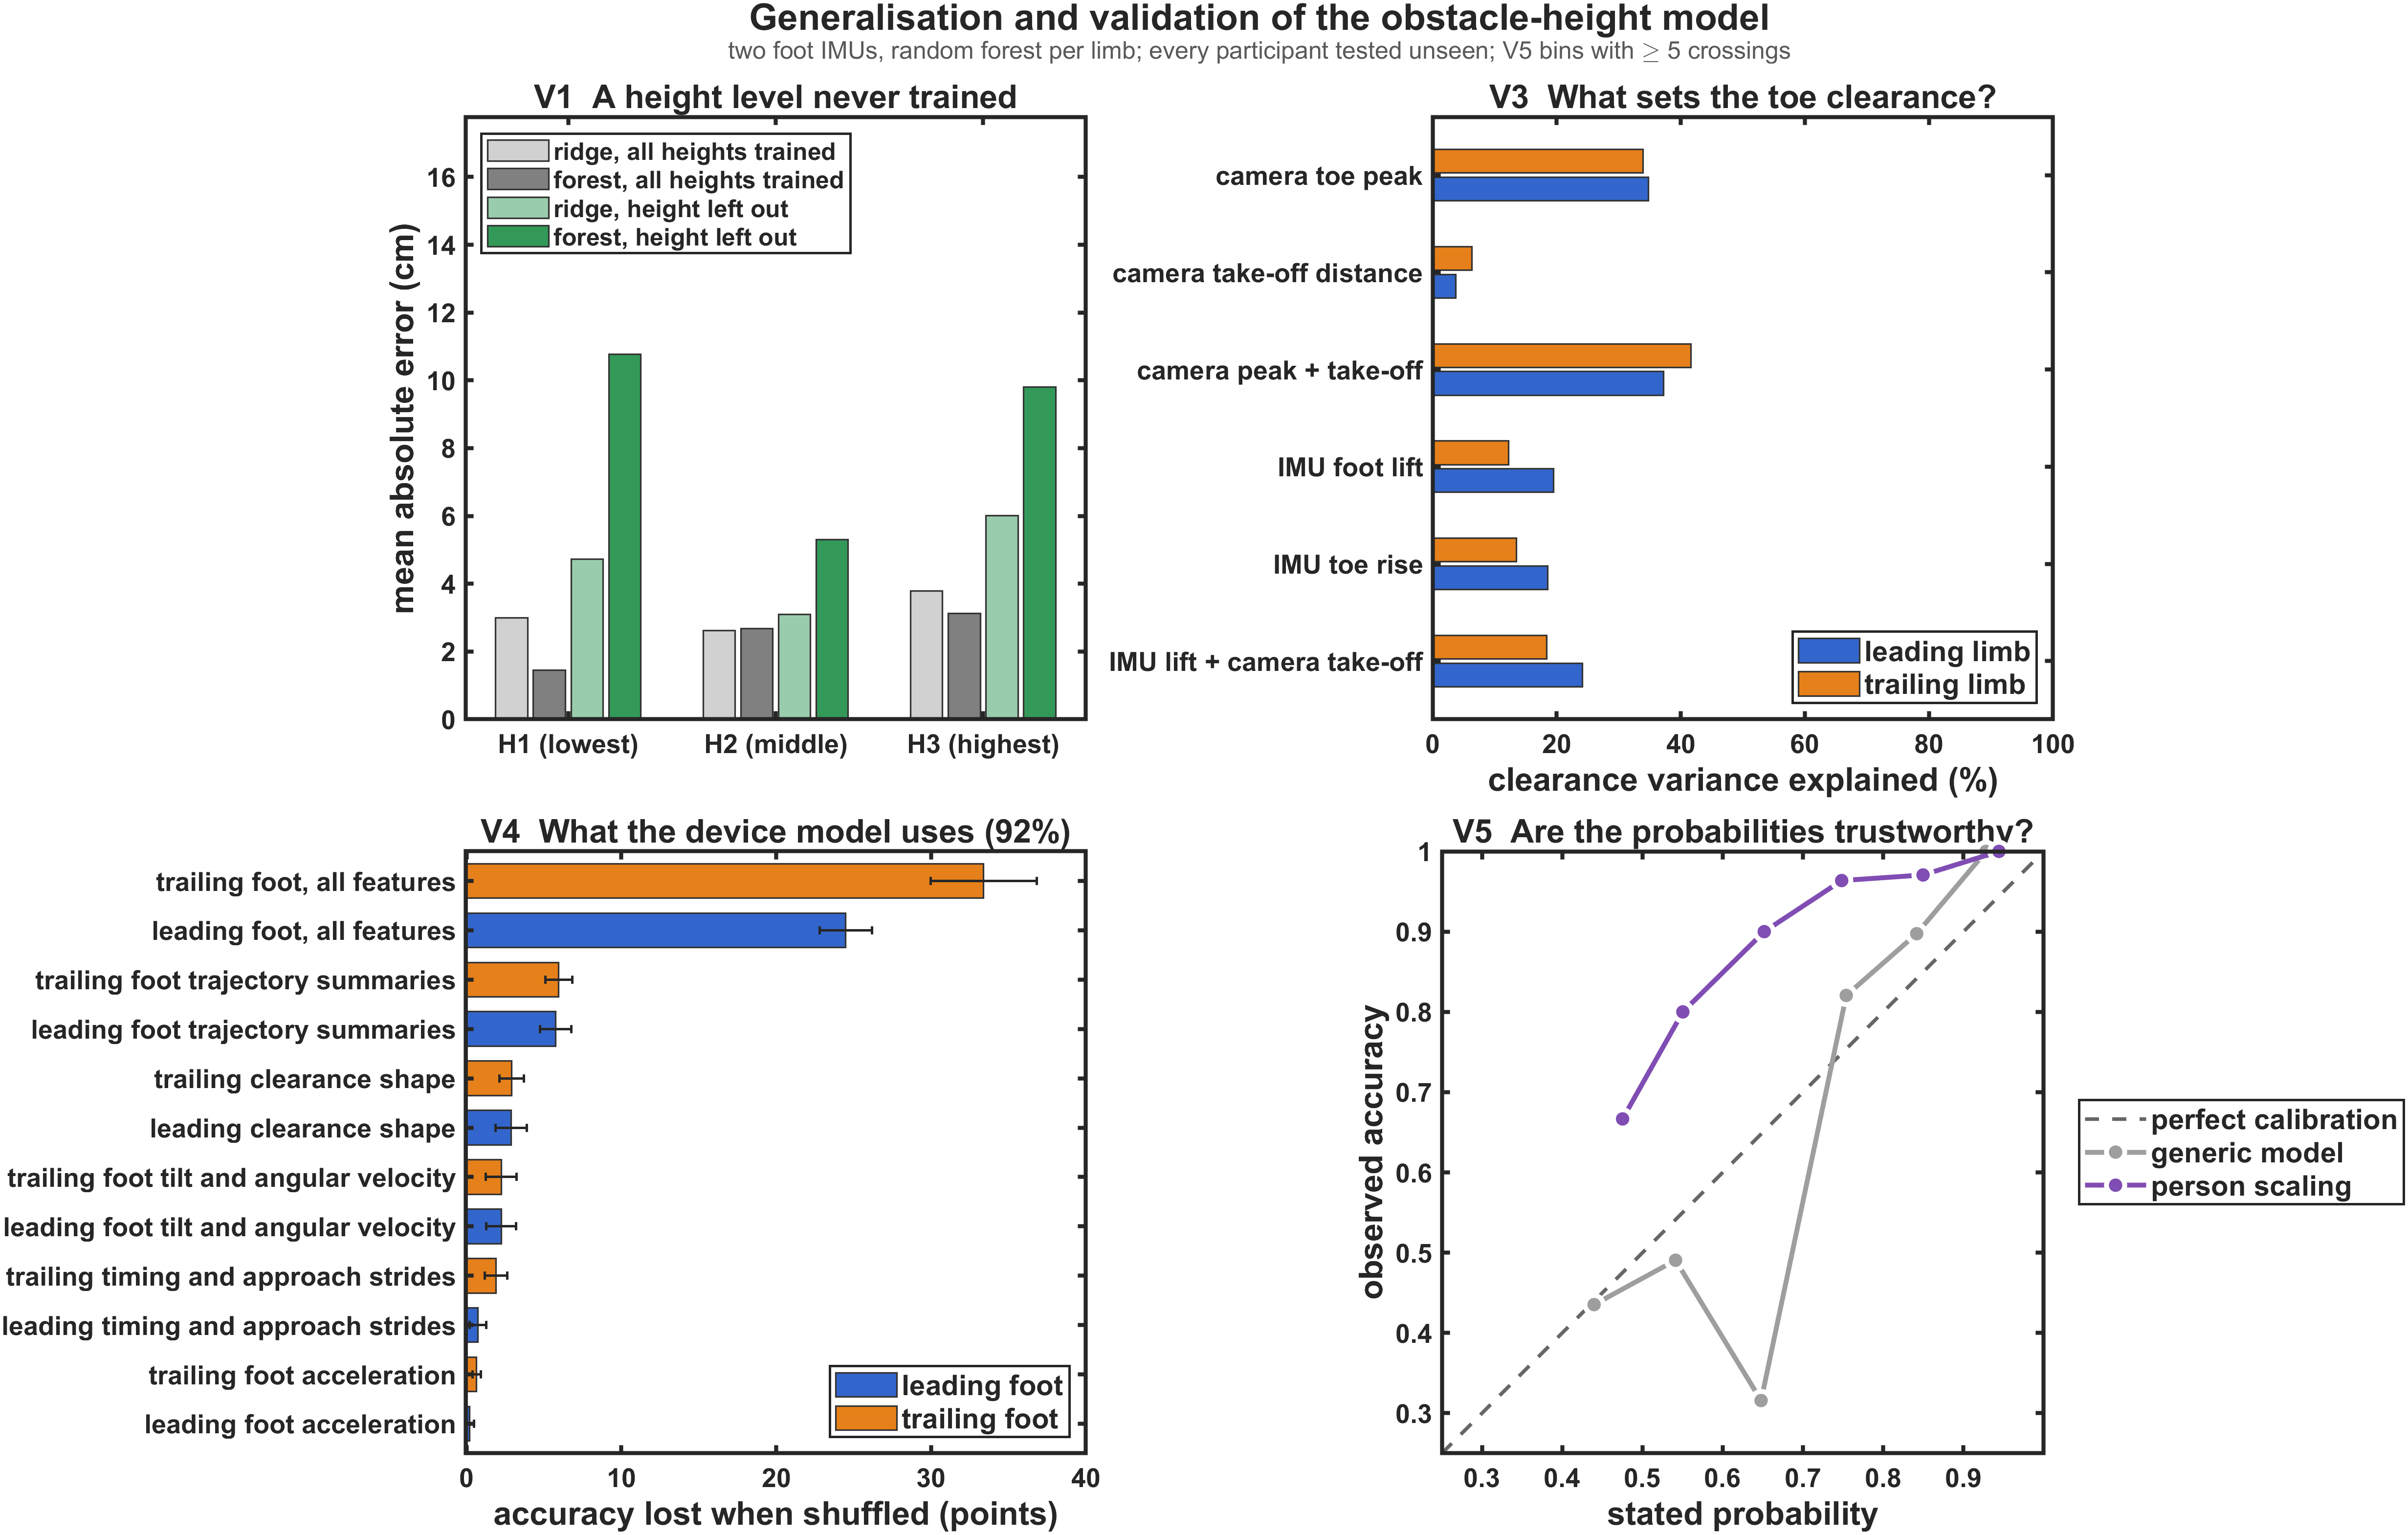
\includegraphics[width=\textwidth]{fig_validate.png}
\caption{Validation. V1: height error when a height level is missing from training (grey = trained on all heights, green = this
height left out; light = ridge, dark = forest). V3: what explains the crossing-to-crossing clearance (blue = leading, orange =
trailing limb). V4: accuracy lost when a feature group of the final model is shuffled (permutation importance). V5: reliability of
the stated probabilities (grey = generic, purple = person scaling, dashed = perfect calibration).}
\label{fig:validate}
\end{figure}


